\documentclass{ctexart}
\usepackage{amsmath}
\usepackage{float}
\usepackage{amssymb}
\usepackage{graphicx}
\usepackage{gbt7714}
\usepackage{wrapfig}
\ctexset{
    % 修改 section。
    section={   
        name={,、},
        number={\chinese{section}}
    }
}

\title{非线性元件的伏安特性研究}
\author{陆知辰-10225301478}
\date{\today}
\graphicspath{{figure/}}

\begin{document}

\begin{titlepage}
  \centering
  % 插入图片
  
\includegraphics[width=0.5\textwidth]{ecnu.png}
  
  % 空行用于调整标题位置
  \vspace*{\baselineskip}
  
  % 标题
  \Huge\textbf{物\quad 理\quad 实\quad 验 \quad (二)}
  % 空行用于调整标题和其他信息之间的间距
  \vspace*{0.3\baselineskip}
  
  % 具体实验名称
  \huge 非线性元件的伏安特性研究
  
  % 空行用于调整时间和其他信息之间的间距
  \vspace*{2\baselineskip}
  
  % 时间
  \large 时间:\today
  
  % 空行用于调整时间和其他信息之间的间距
  \vspace*{\baselineskip}
  
  % 创作人
  \large 创作人:陆知辰
  
  % 空行用于调整创作人和学号之间的间距
  \vspace*{\baselineskip}
  
  % 学号
  \large 学号:10225301478
  
\end{titlepage}
\newpage
\tableofcontents
\newpage
\section{实验摘要}
  \subsection{实验概要}
  伏安特性描述了电子元件在两端通过直流电压和通过元件的电流之间的关系。

  非线性元件就是在电子元件两端通过直流电压和通过元件的电流之间的关系不是线性的。
  现实中有很多电子元件都是非线性的。就如实验中将要用到的二极管、灯泡中的钨丝等都是非线性元件。
  非线性元件的电阻总是与一定的物理过程相联系,如发热、发光和能级跃迁等。

  本次实验主要研究非线性元件电路设计和测量导通方法。

  \subsection{实验目的}
  1.\quad 了解测量电路中电路元件的选取方法、调节方法。

  2.\quad 掌握待测元件的基本特性,能测量二极管的正向导通电压。
  
  3.\quad 掌握非线性元件伏安特性的测量电路和研究方法。

\section{实验原理}
  \subsection{伏安特性}
  \begin{figure}[t]
    \centering
    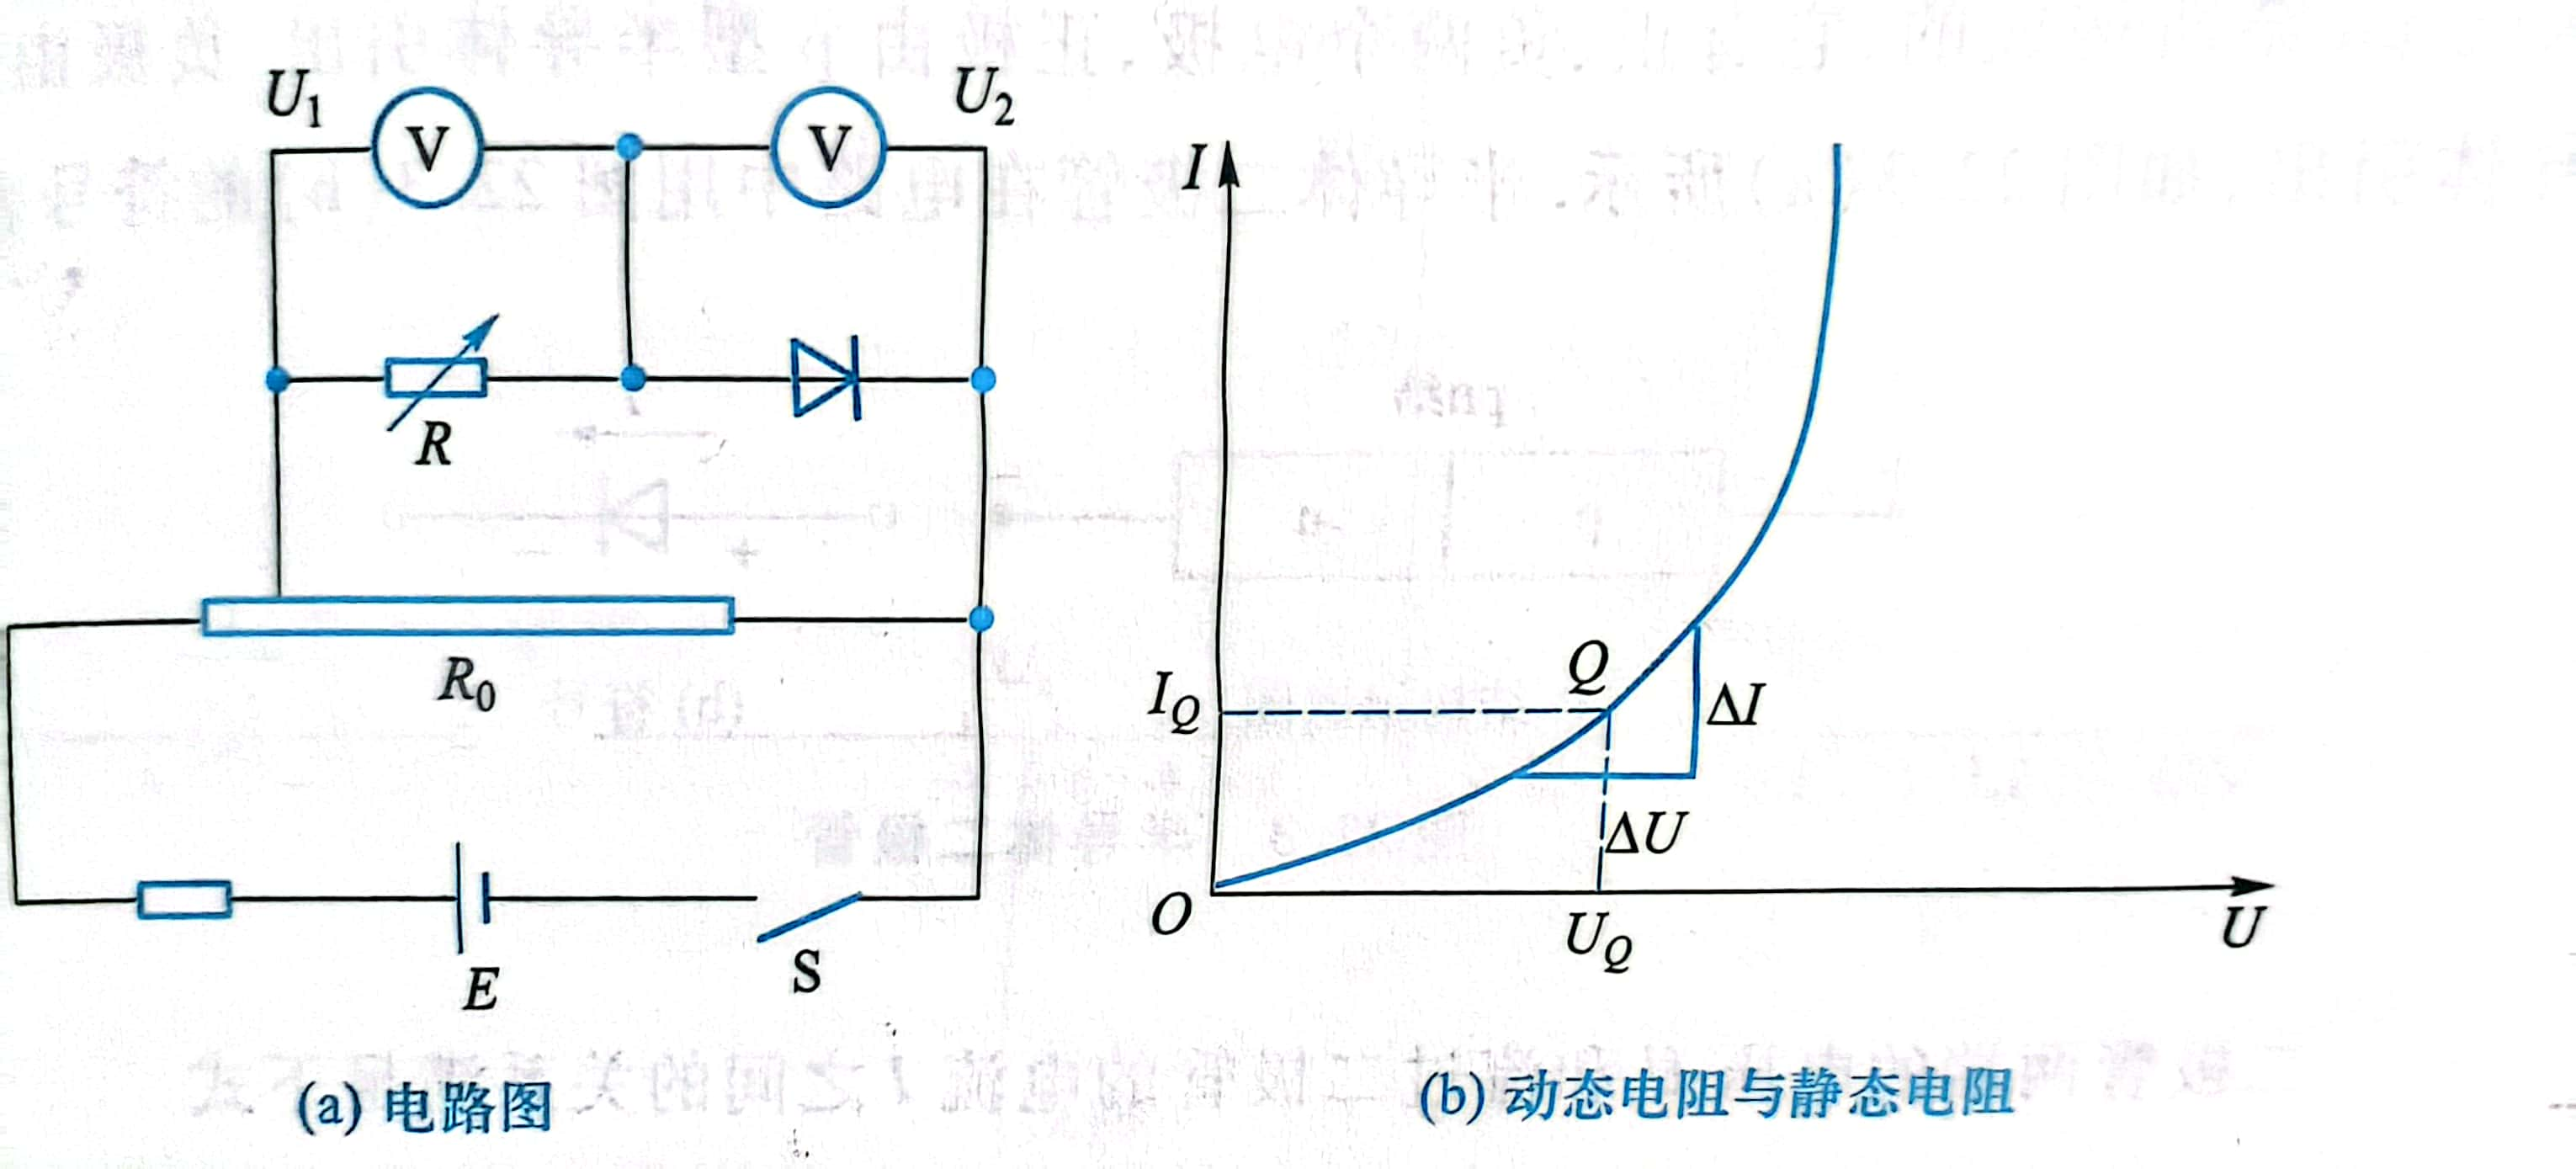
\includegraphics[width=1\textwidth]{fuantexingdianlu.jpg}
    \caption{伏安特性测试电路及非线性元件伏安特性曲线}\label{fuantexingdianlu}
  \end{figure}
  非线性元件的伏安特性可以使用如图\ref{fuantexingdianlu}。电路通过调节$R_{0}$
  来调节$R$以及非线性元件分的电压。再通过$R$的阻值大小来最终控制非线性元件两端
  的电压。电子元件并联的电压表电阻具有较大内阻,在测量这类电阻较低的电子元件的时候
  引入的系统误差较小,可以忽略不计。

  根据欧姆定律$R=\frac{U}{I}$,通过图\ref{fuantexingdianlu}中所展示的电路,由
  待测元件两侧的电压$U$以及电流$I$可以计算得到待测元件的阻值$R$。但是非线性元件的
  阻值$R$并不是一个定值,所以当描述非线性元件的电阻的时候需要指明工作的状态,即指出
  工作电流或者工作电压。

  非线性元件的电阻可用两种方式表示。第一种为静态电阻,用$R_{D}$表示;另一种为动态
  电阻,用$R_{rp}$表示。动态电阻等于工作点附近的电压改变量和电流改变量的比值,可以
  通过伏安特性曲线得到。如图\ref{fuantexingdianlu}展示的那样,在$Q$点附近的
  静态电阻和动态电阻可以表示为
  \begin{equation}
    R_{D}=\frac{U_{Q}}{I_{Q}}
  \end{equation}
  \begin{equation}
    R_{rp}=\frac{\Delta U}{\Delta I}
  \end{equation}

  \subsection{白炽灯灯丝的伏安特性}
  \begin{figure}[t]
    \centering
    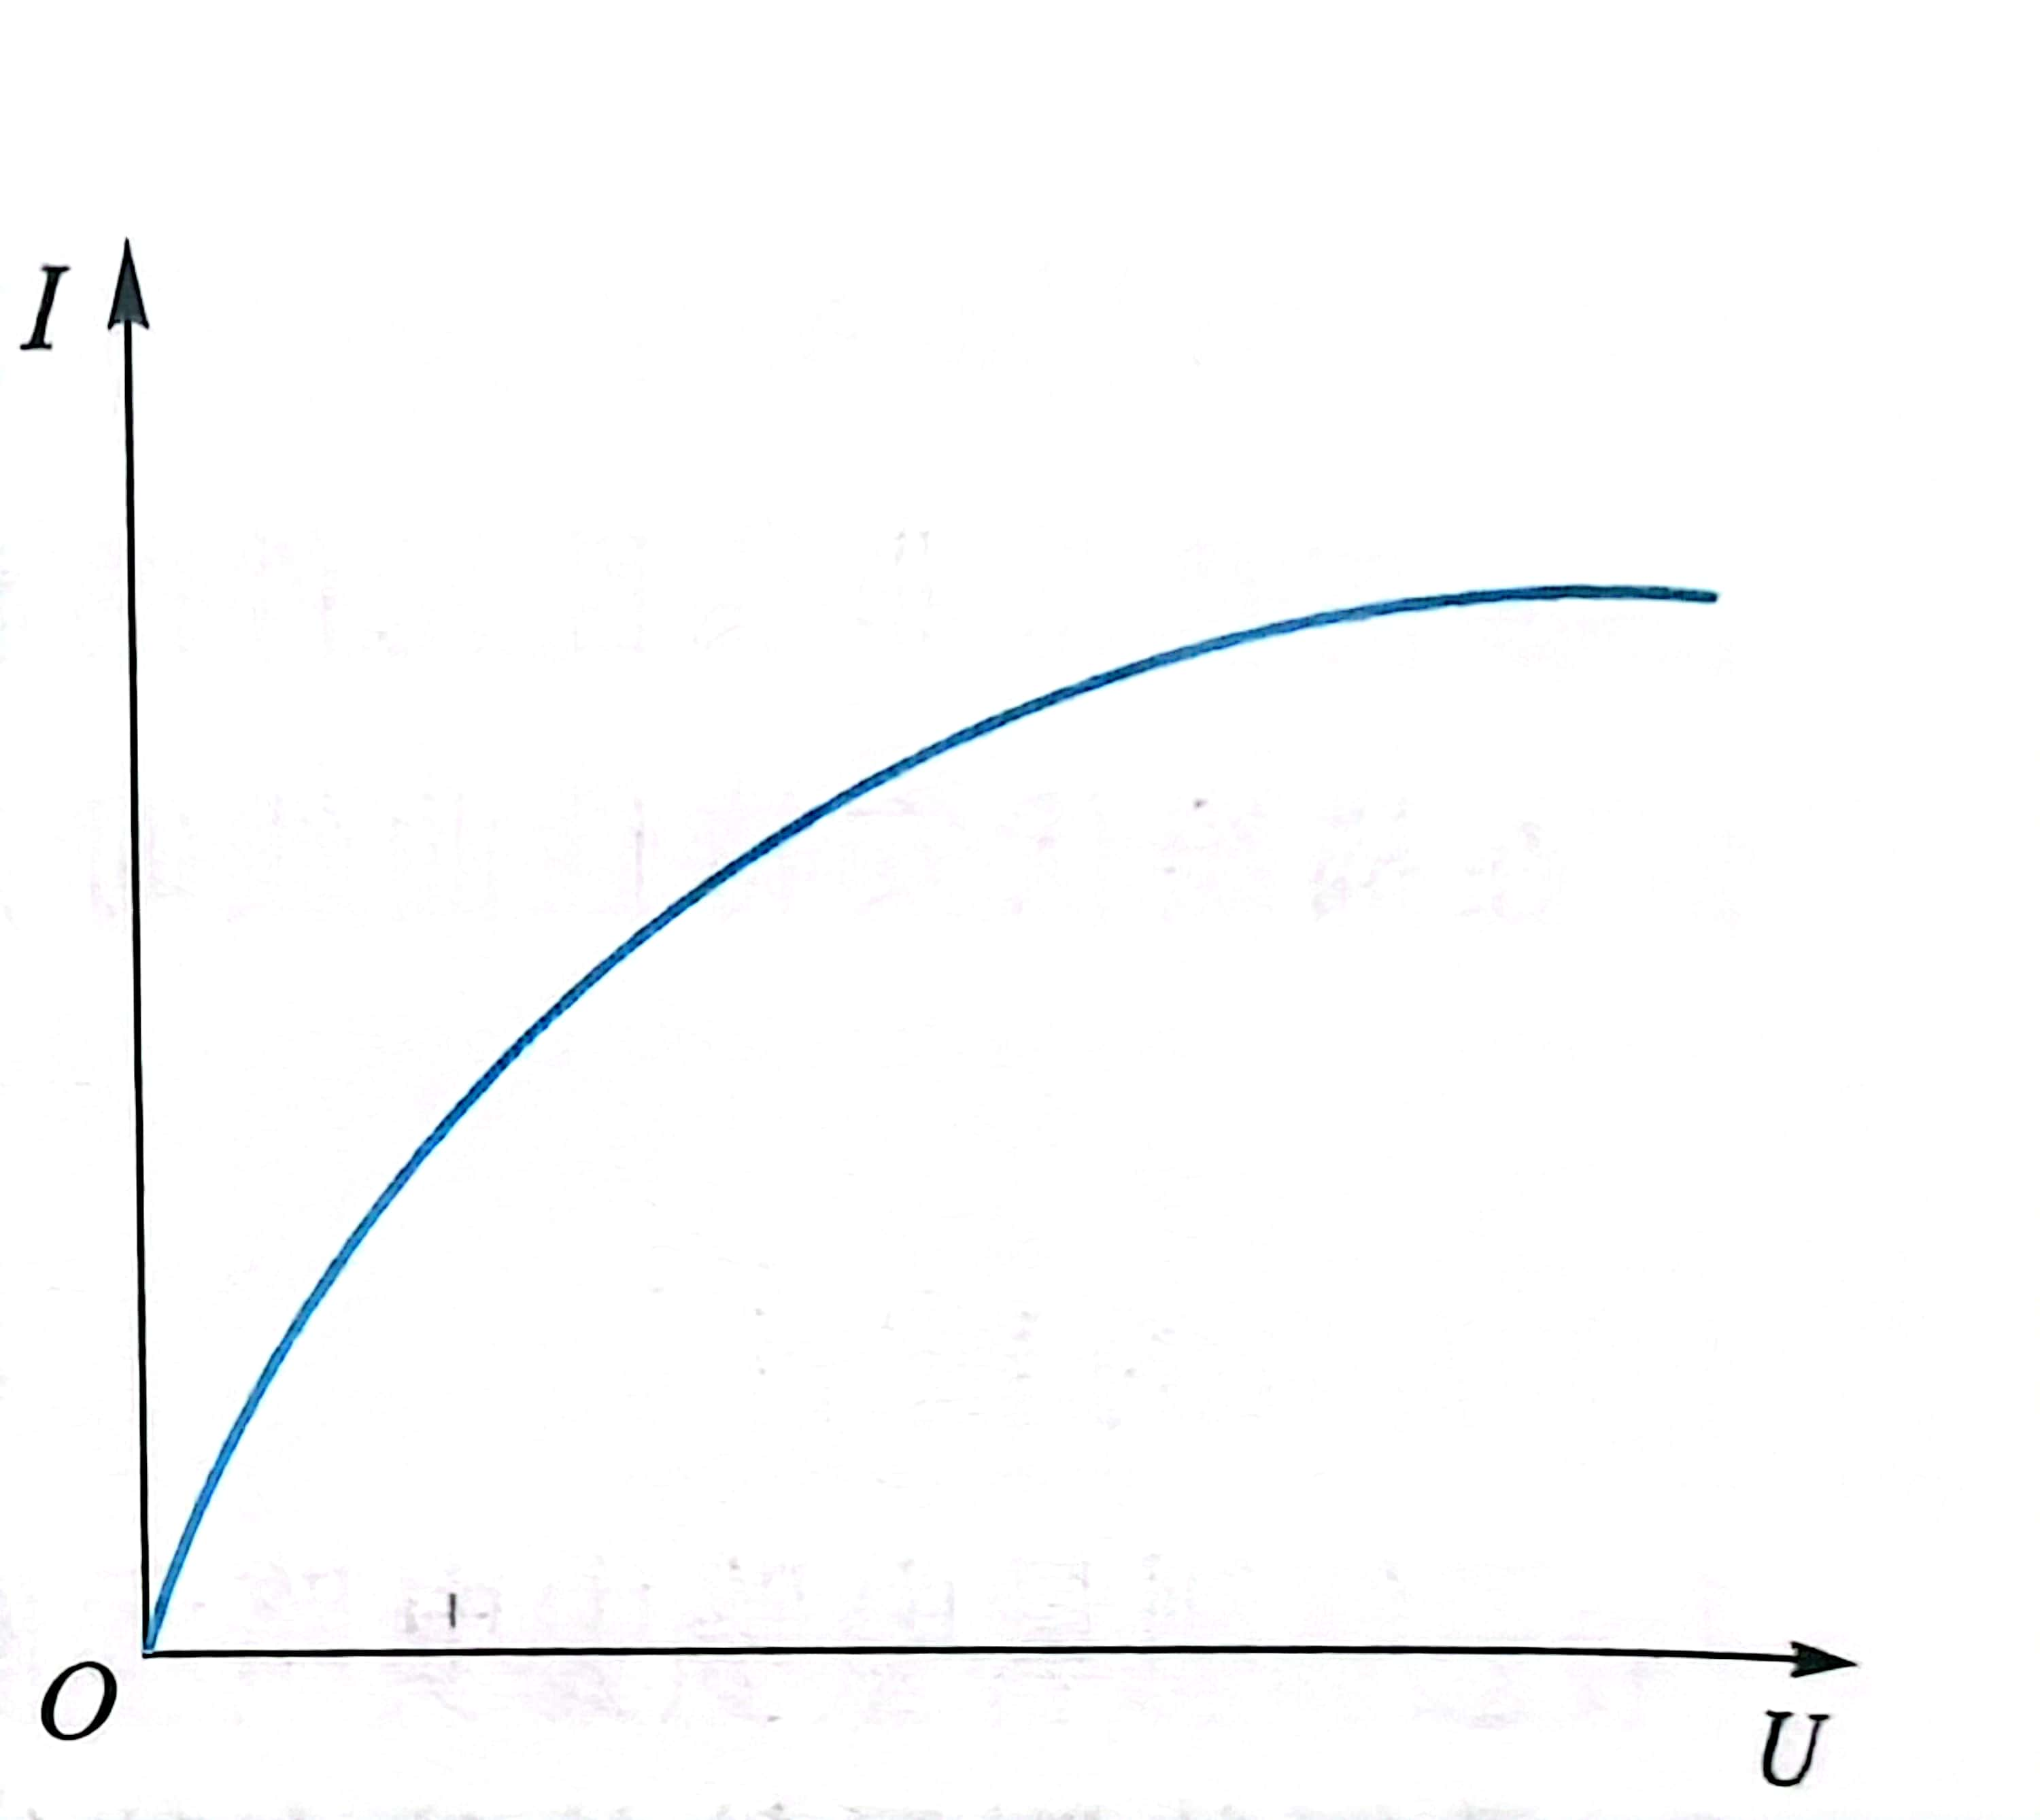
\includegraphics[width=0.5\textwidth,height=0.3\textheight]{dengpaofuantexing.jpg}
    \caption{灯泡伏安特性曲线}\label{dengpaofuantexing}
  \end{figure}
  钨丝类的灯泡发光后,灯丝的电阻会由于发热随着温度升高而增。这意味着通过灯丝的电流越大,
  灯丝发热越严重,电阻也越大。由于温度差异而产生的电阻差异可能相差几倍甚至几十倍。灯泡
  两端的电压以及通过灯泡的电流之间的关系如图\ref{dengpaofuantexing}所示。它们之间的关系
  可以表示为
  \begin{equation}\label{shidengpaofuantexing}
    U=KI^{n}
  \end{equation}
  其中$K$和$n$是和灯泡有关的参数。

  将式\ref{shidengpaofuantexing}两端取对数,将非线性的关系转化为线性关系
  \begin{equation}
    \ln U=\ln K+n\ln I
  \end{equation}
  通过实验测量$U$和$I$关系,再进行作图法或者最小二乘法确定$K$和$n$的值。

  \subsection{半导体二极管的伏安特性}
  \begin{figure}[t]
    \centering
    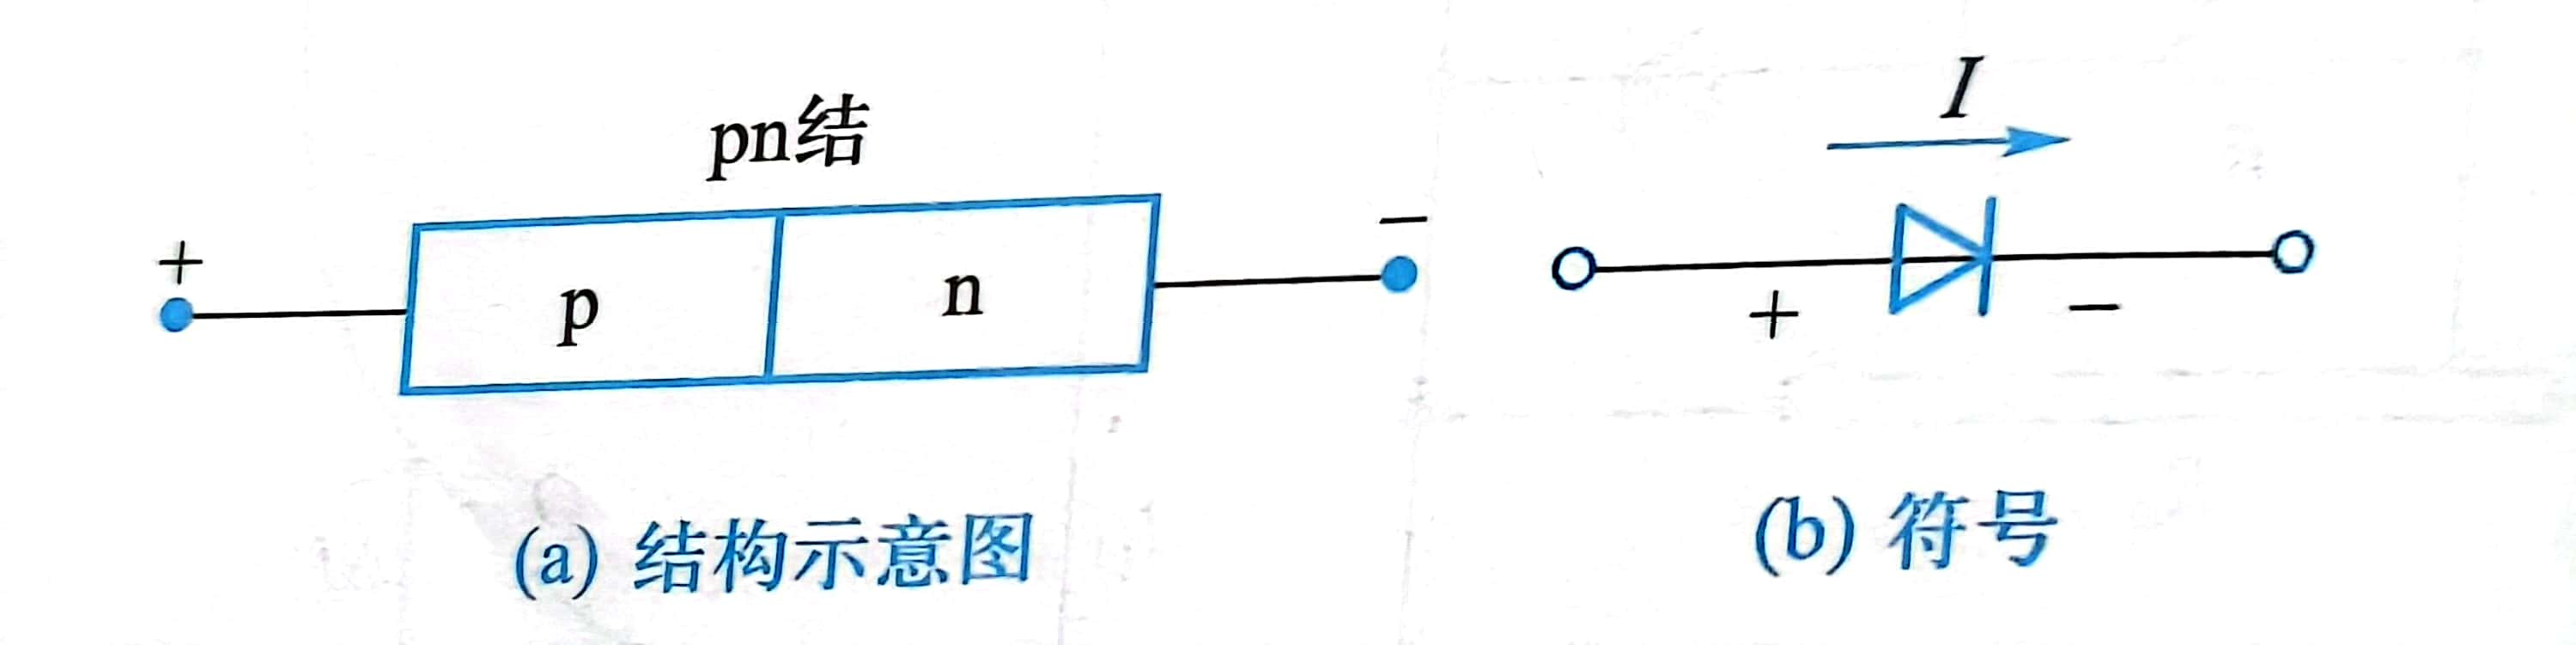
\includegraphics[width=1\textwidth,height=0.3\textheight]{bandaoti.jpg}
    \caption{半导体二极管示意图}\label{bandaoti}
  \end{figure}
    \subsubsection{半导体二极管介绍}
    半导体二极管又称为晶体二极管,也是非线性元件。在电路中二极管具有单向导电性。
    由于能够控制电流流过的方向,所以二极管能够在电路中发挥很多作用,比如整流、检波、
    限幅、元件保护以及数字电路中作为开关的元件。
    二极管是通过两种不同导电性能的半导体进行结合后产生的,这两种半导体分别为
    $n$型半导体以及$p$型半导体。这两种半导体结合后会产生$PN$结。正极由$p$型半导体引出,
    负极由$n$型半导体引出,最终产生的结构以及电路中的示意如图\ref{bandaoti}。
    \begin{equation}\label{erjiguan}
      I=I_{s}(e^{ \frac{qU}{kT}}-1)
    \end{equation}

    \subsubsection{半导体二极管伏安特性}
    二极管两端的电压$U$和流过二极管的电流$I$之间的关系满足式\ref{erjiguan}。
    式子中的$q=1.602\times 10^{-19}C$为电子电荷量的绝对值,
    $k=1.381\times 10^{-23}J/K$为玻尔兹曼常数,$T$为热力学温度,$I_{s}$为反向饱和电流。
    \begin{figure}[tbh]
      \centering
      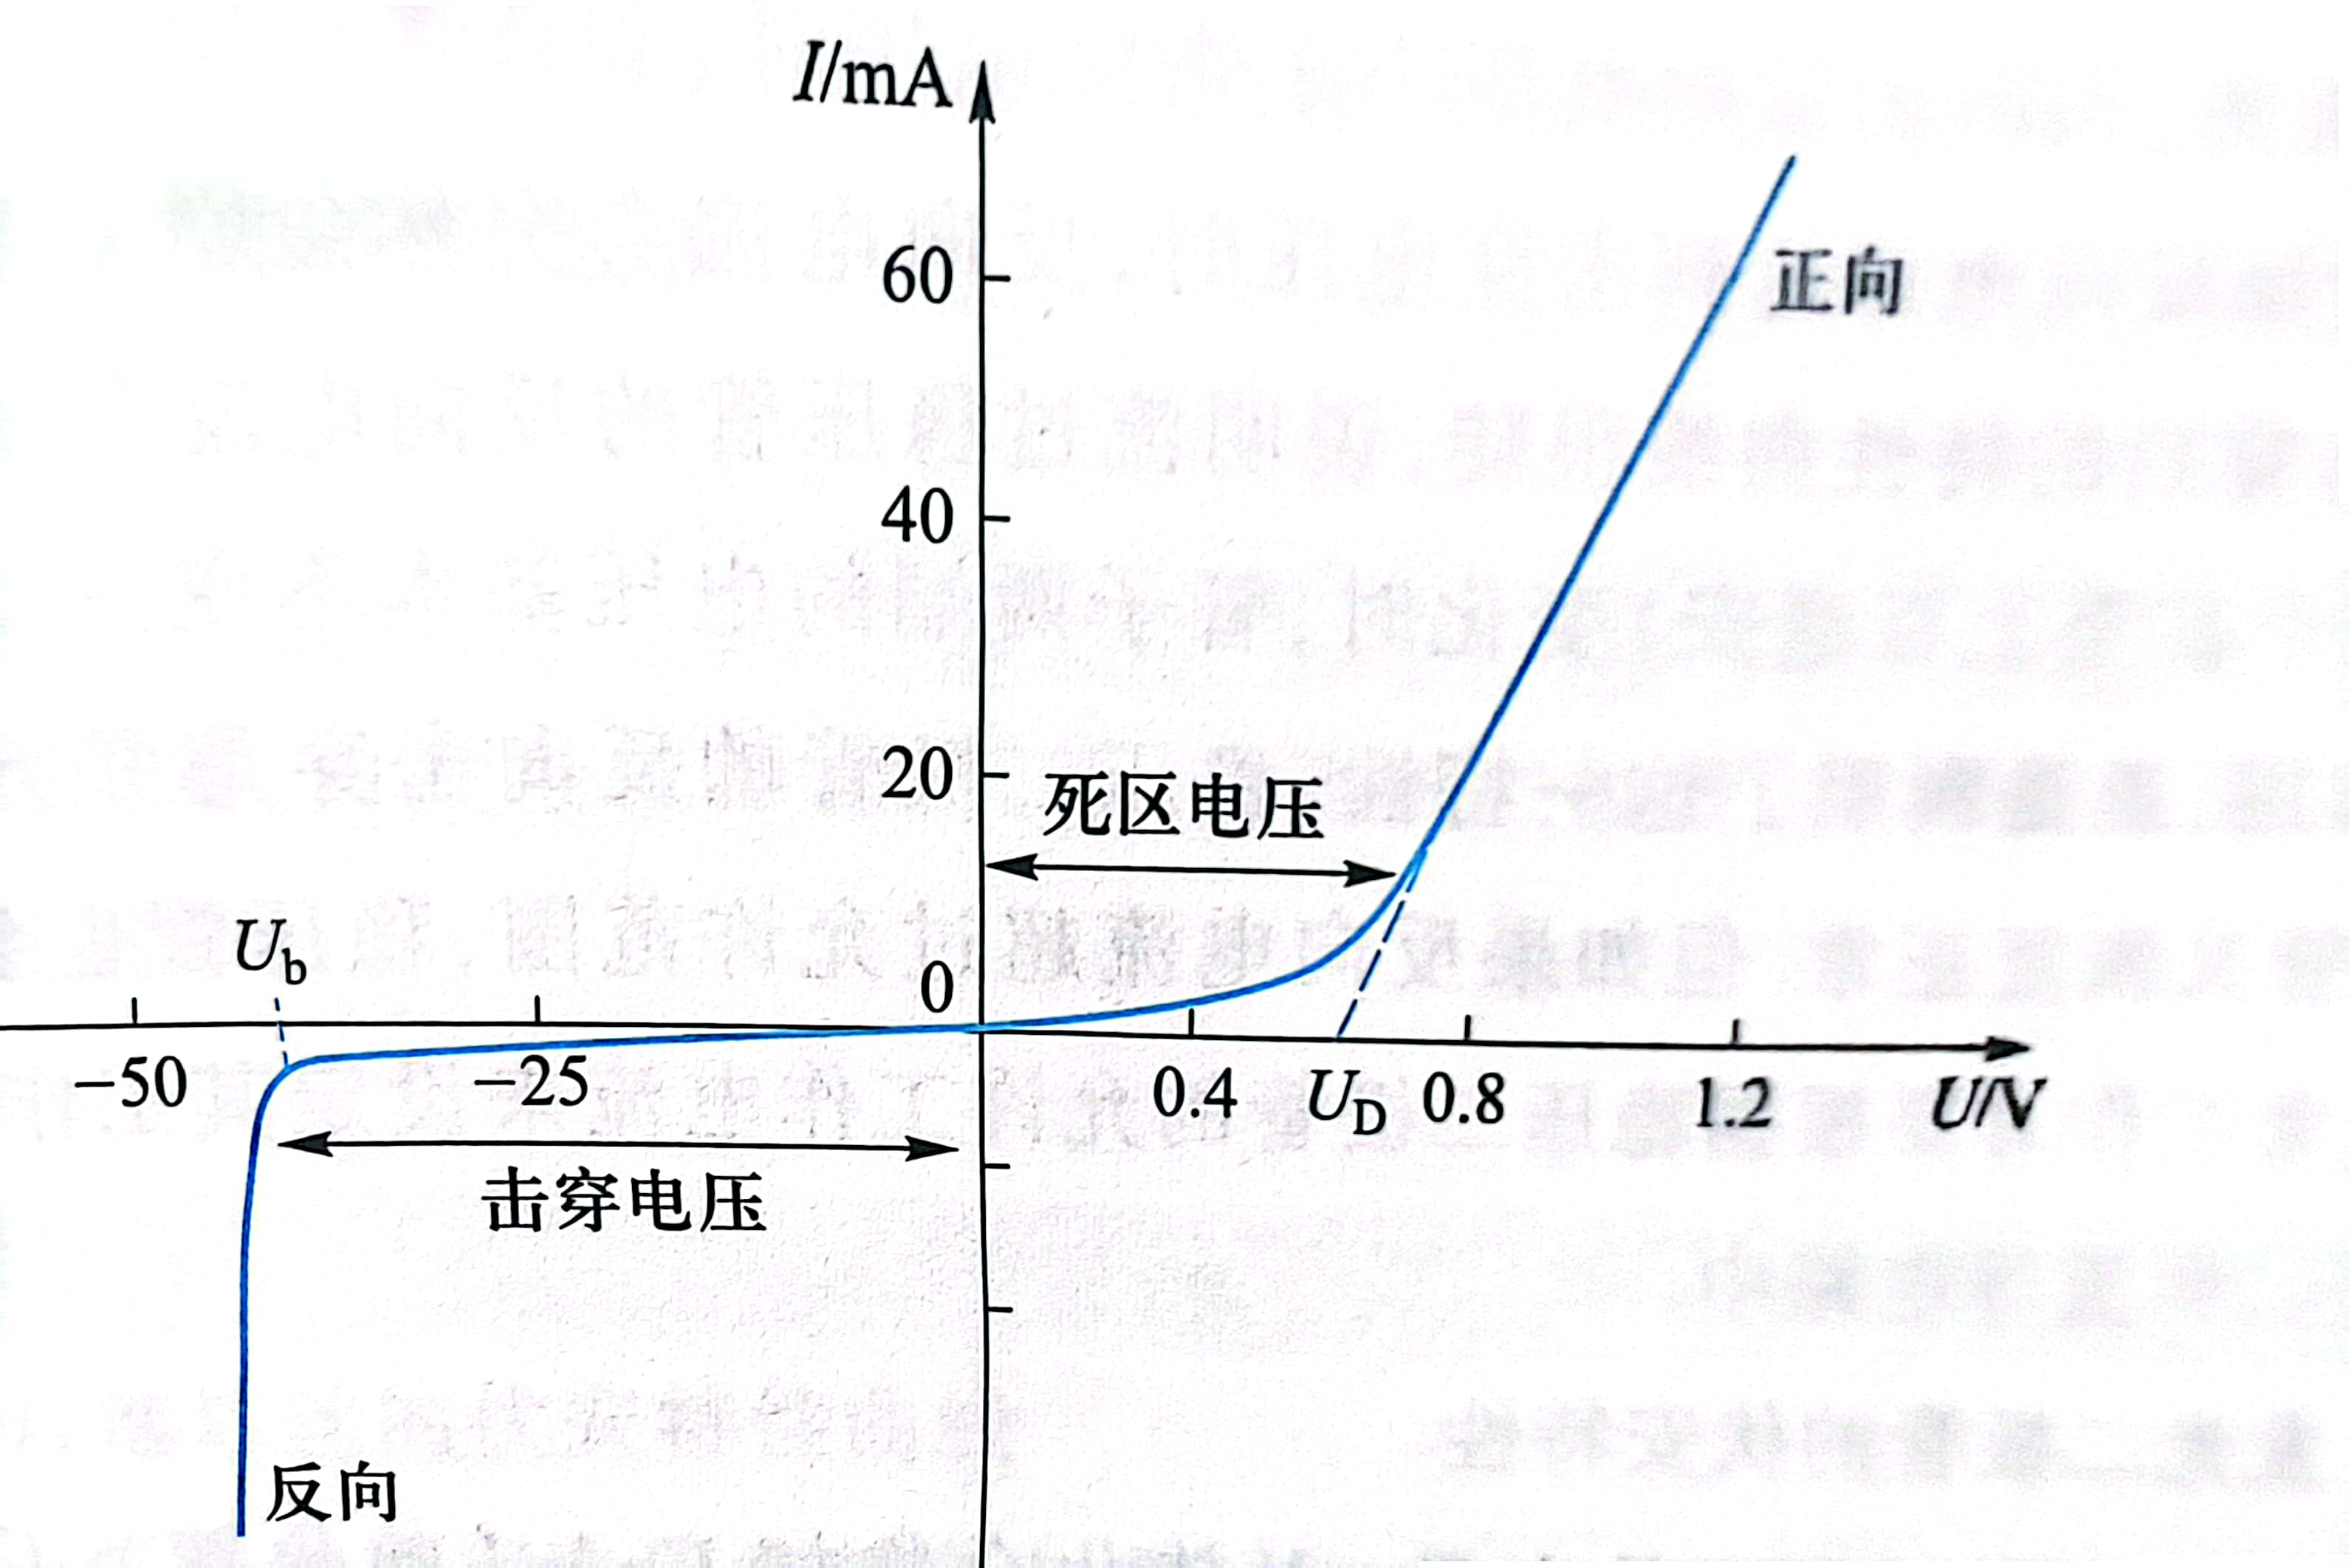
\includegraphics[width=1\textwidth]{erjiguanfuantexing.jpg}
      \caption{半导体二极管伏安特性曲线}\label{erjiguanfuantexing}
    \end{figure}
    
    半导体二极管的主要特点就是单向导电性,其伏安特性曲线如图\ref{erjiguanfuantexing}。由此可以看出,
    二极管在正向电压较小的时候,电流值较小,而一旦电压增加到超过阈值电压$U_{D}$之后,正向电流开始明显
    增大,随着电压增加电流也在急速增大,伏安特性曲线近似可以看为一条直线。将该直线反向延长和$x$轴
    相交于$U_{D}$,$U_{D}$为正向导通阈值电压

    而对半导体二极管加上反向电压的时候,反向电流极小而且随电压变化缓慢,但当反向电压最终超过击穿
    电压时候$U_{b}$,电流将急剧增大,二极管被击穿后仍可以恢复到正常工作,但是由于发热等原因实际上
    仍然会对二极管产生不可逆的损害,最终造成二极管永久损坏。

  \subsection{稳压二极管的伏安特性}
  稳压二极管是一种特殊的硅二极管,伏安特性曲线如图\ref{wenyafuantexing}
  \begin{figure}[tbh]
    \centering
    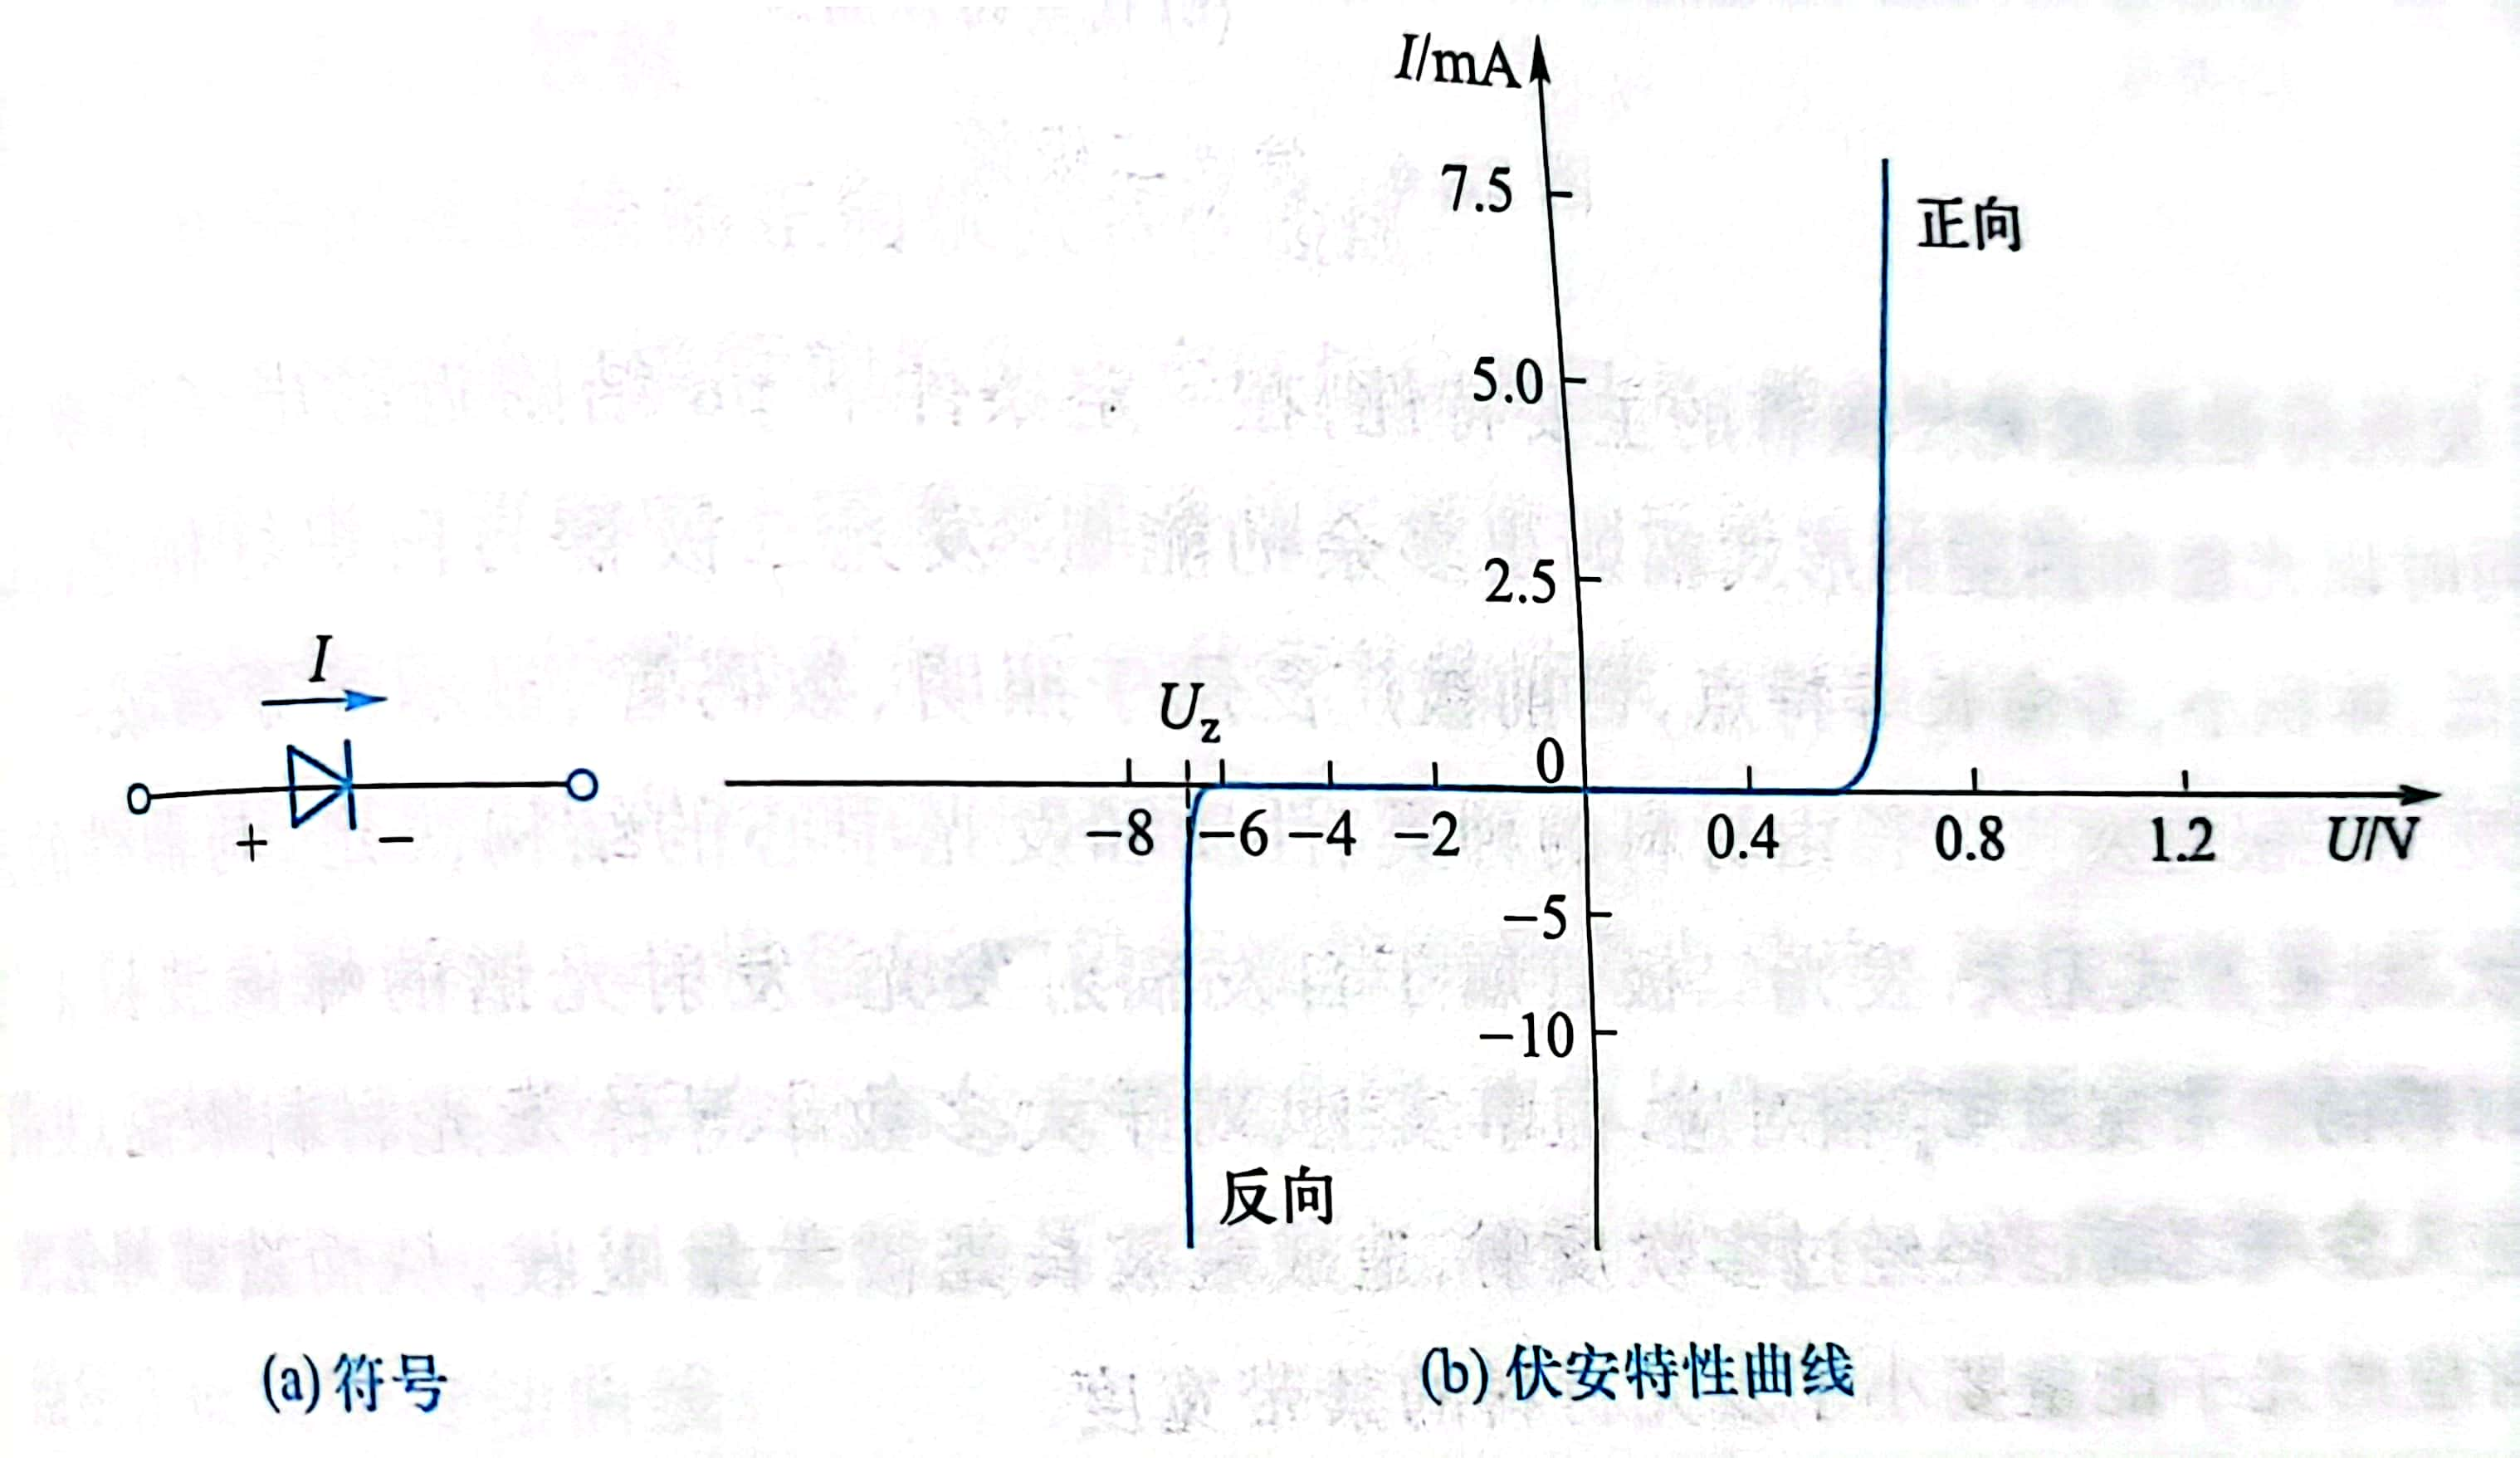
\includegraphics[width=1\textwidth]{wenyafuantexing.jpg}
    \caption{稳压二极管伏安特性曲线}\label{wenyafuantexing}
  \end{figure}
  稳压二极管的伏安特性曲线和普通二极管的和普通二极管类似,只是反向特性曲线较普通二极管更陡。

  对于稳压二极管而言,当电压小于反向击穿电压的时候,它和普通二极管一样。但是一旦电压大于反向击穿
  电压,则在电压增加一个微小量后电流将产生巨大的变化,这说明在很大的电流范围内需要的电压是近似
  不变的。因为这个特性,稳压二极管可以在电路中作为稳压的器件。同时稳压二极管的反向击穿是可逆的,
  当反向击穿电压消失后稳压二极管优惠回复正常。但是和普通的二极管一样,反向击穿是有允许的电压范围的,
  稳压二极管也是一样,如果反向电流超过的了允许范围,则稳压二极管会一样一位电流过大而发热而损坏。
  
  由于具有以上特性,稳压二极管一般用在稳压或者恒流的电路中。

  \subsection{发光二极管的伏安特性}
  \begin{figure}[t]
    \centering
    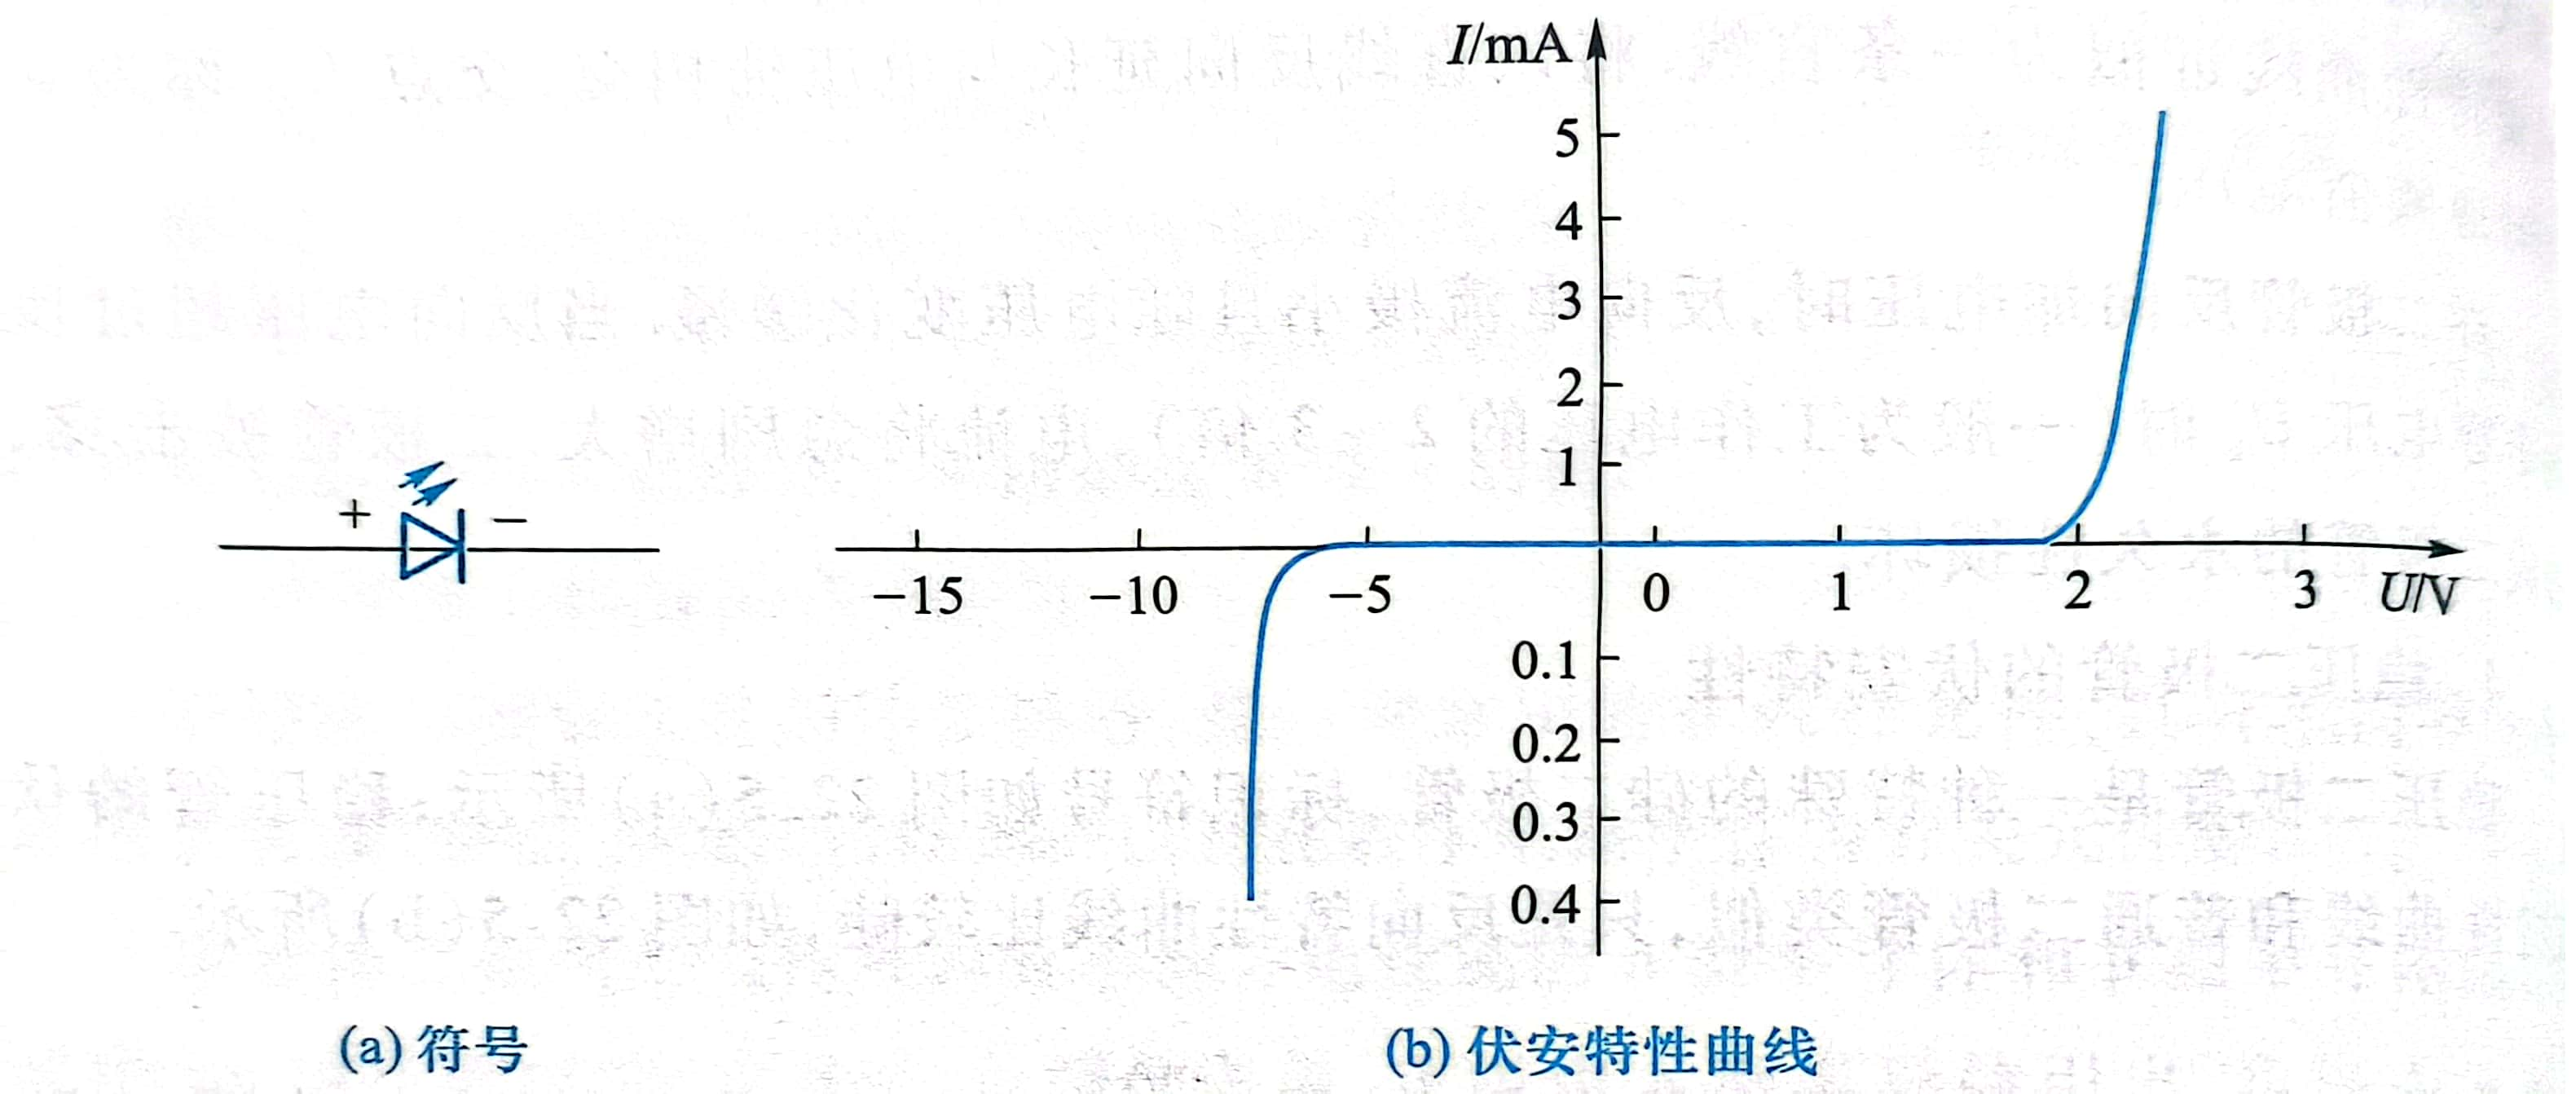
\includegraphics[width=1\textwidth]{faguangfuantexing.jpg}
    \caption{发光二极管伏安特性曲线}\label{faguangfuantexing}
  \end{figure}
  发光二极管,也就是常说的LED一般是由$III-V$族化合物如$GaAs$、$GaP$、$GaAsP$等半导体材料制成的,发光二极管在电路中的符号如
  图\ref{faguangfuantexing}中展示的那样。发光二极管的核心依旧是pn结,因此它具有一般pn结有的特性,它的伏安特性曲线和普通的
  二极管类似。
  
  发光特性是发光二极管的主要特性,在一定条件下pn结附近的的电子和空穴会复合,同时以光能和热能的形式向外辐射出多余的能量。发光
  二极管和白炽灯相比,具有功耗低,体积小,寿命长的特点,目前被广泛应用在照明、数码管、显示屏等电子领域。

  对于发光二极管而言,发光的波长由材料的种类、性质和发光中心的结构相关。但是和器械的封装方式、形状无关。发光二级管属于
  自辐射发光,所以发射光谱的峰值波长$\lambda$和发光材料的禁带宽度$E_{g}$相对应。但是事实上对于大多数半导体发光材料而言,发射光进入
  空气之前已经经历了多次反射,所以造成了短波长光被大量吸收,从而造成峰值波长相对应的光子能量要小于发光材料的禁带宽度。

  辐射跃迁所发出的光子的峰值波长$\lambda$可以由式\ref{fenzibochang}来计算
  \begin{equation}\label{fenzibochang}
    \lambda \approx 1240/E_{g} \quad (nm)
  \end{equation}

\section{实验装置器材介绍}
稳压电源、电阻箱、可变电位器、九孔板、待测试二极管、待测试稳压二极管、待测试小灯泡、导线若干

\section{实验内容及实验步骤}
  \subsection{测量普通二极管的正向伏安特性曲线}

  \begin{figure}[b]
    \centering
    \begin{minipage}[b]{0.48\textwidth}
      \centering
      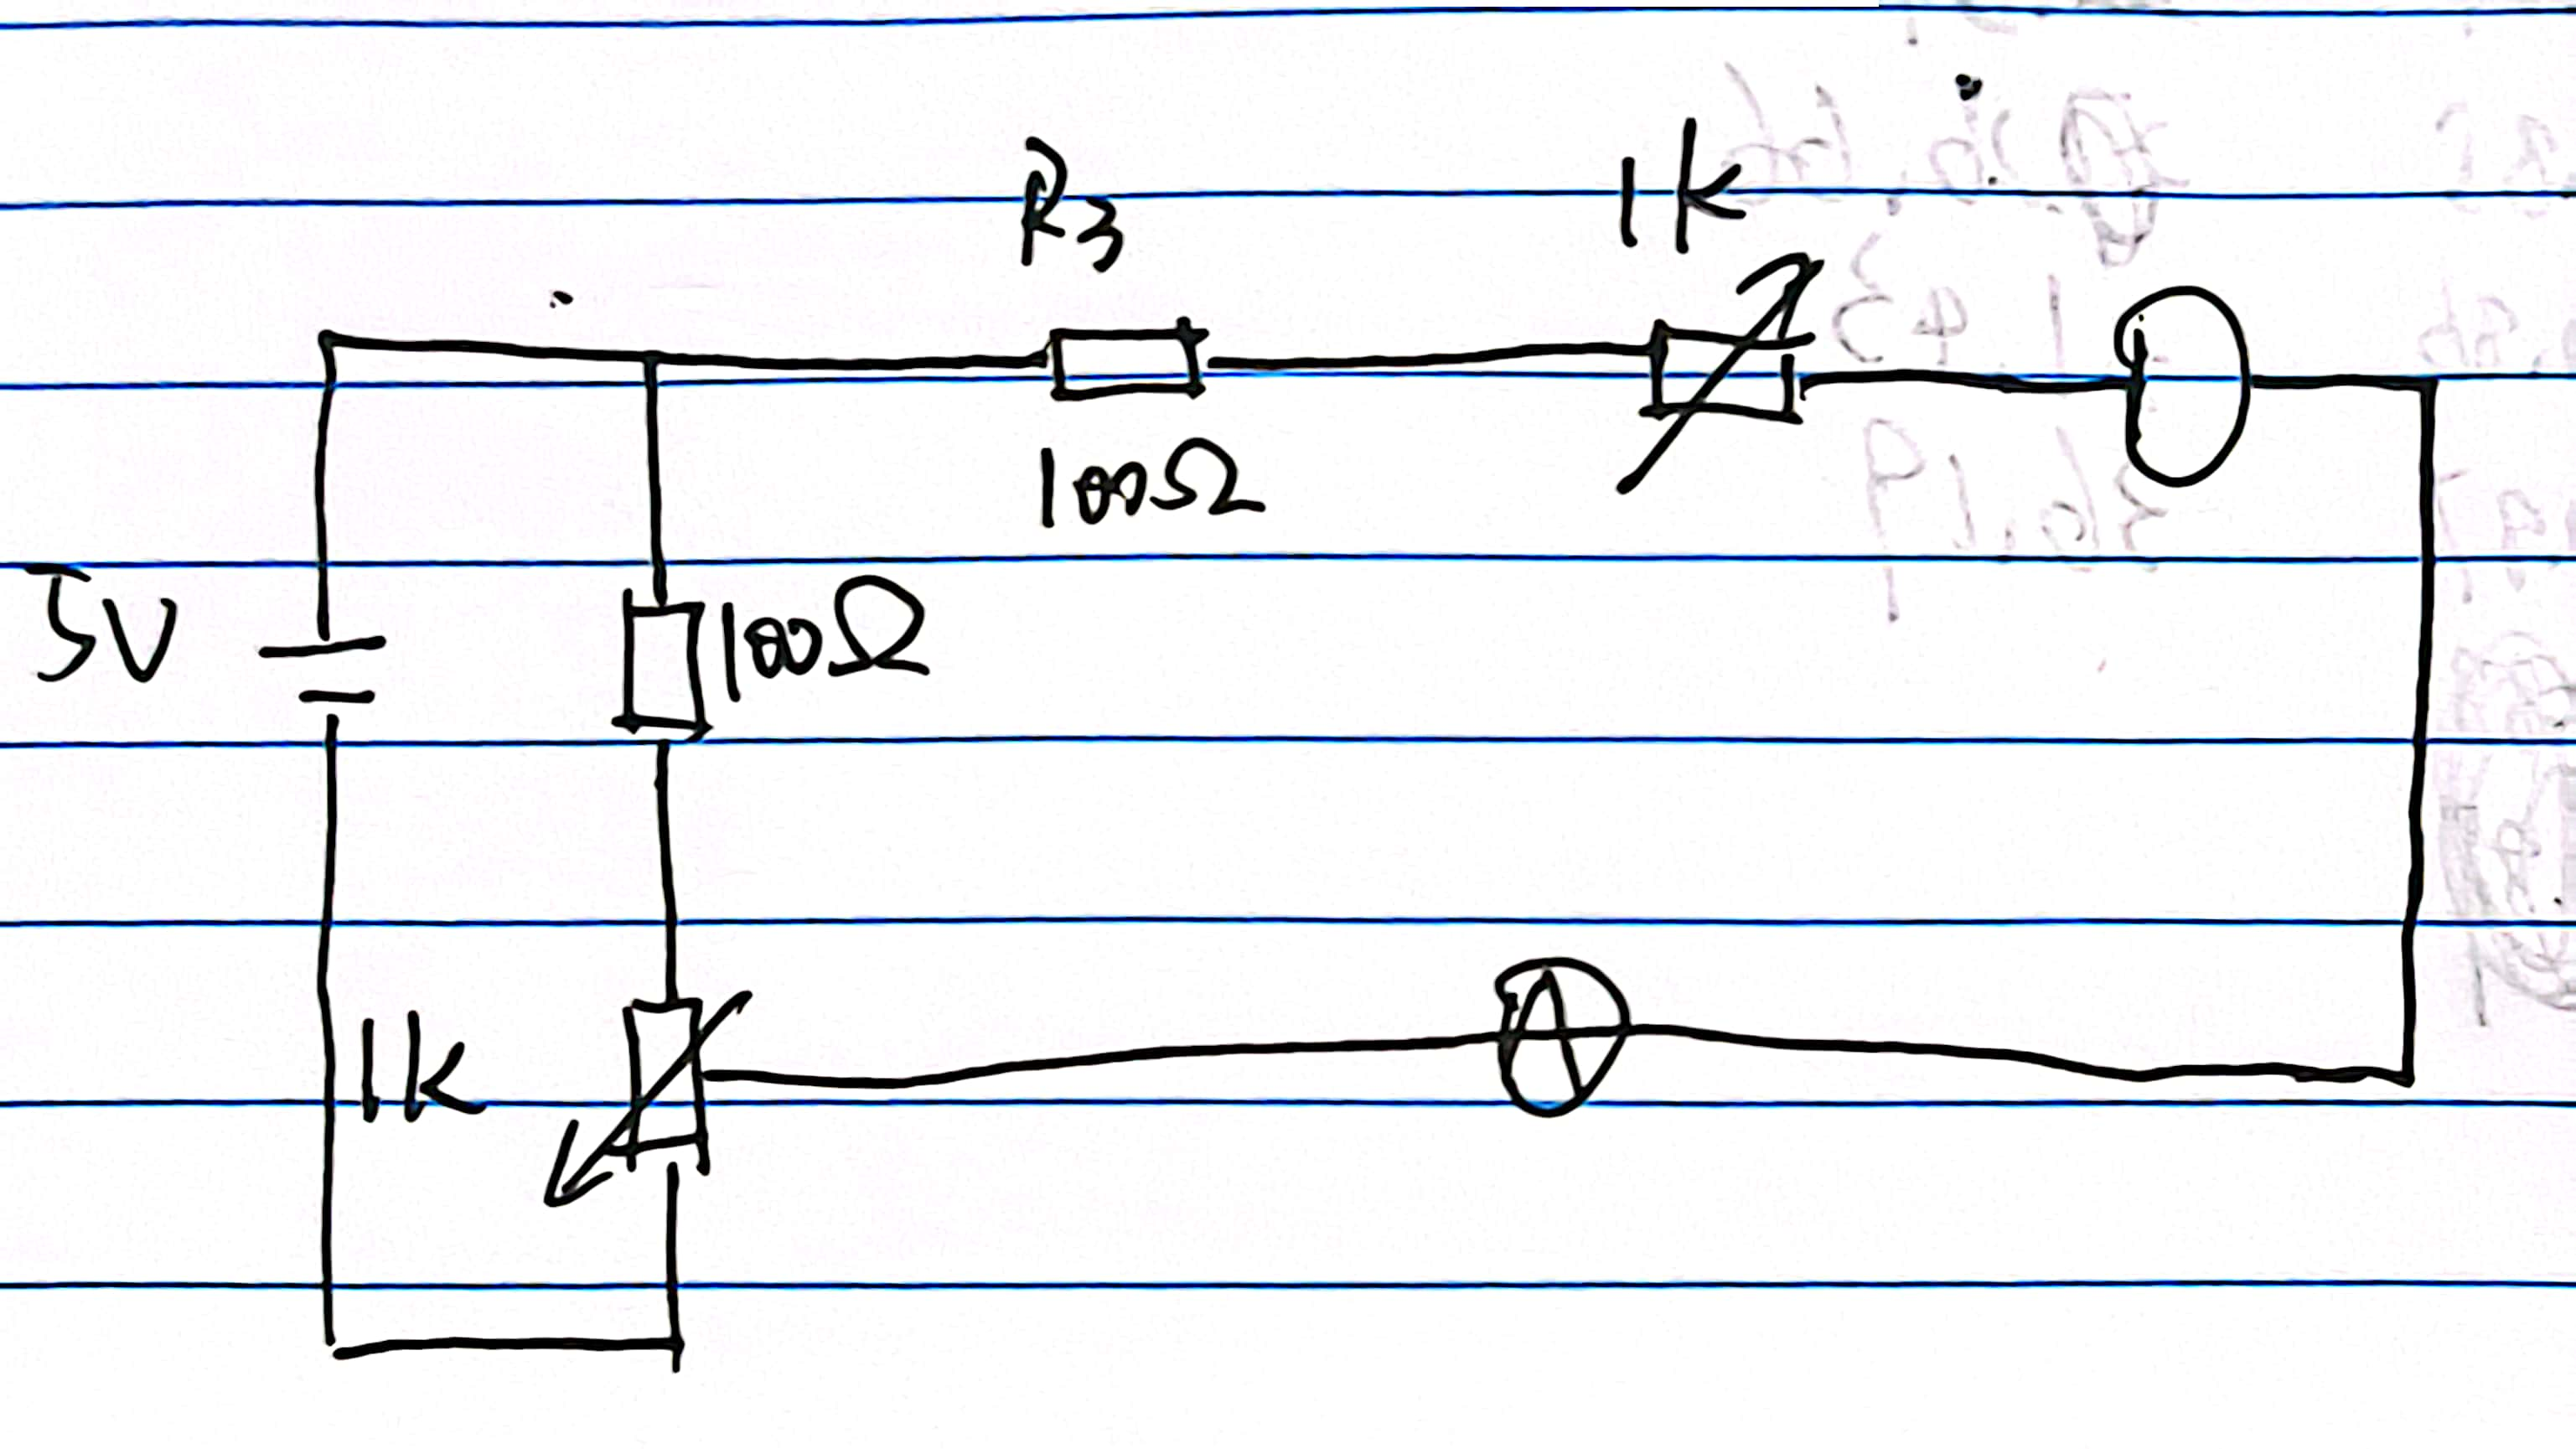
\includegraphics[width=0.46\textwidth]{zhengxiangdianlu.jpg}
      \caption{二极管正向连通电路示意图}\label{zhengxiangdianlu}
    \end{minipage}
    \begin{minipage}[b]{0.48\textwidth}
      \centering
      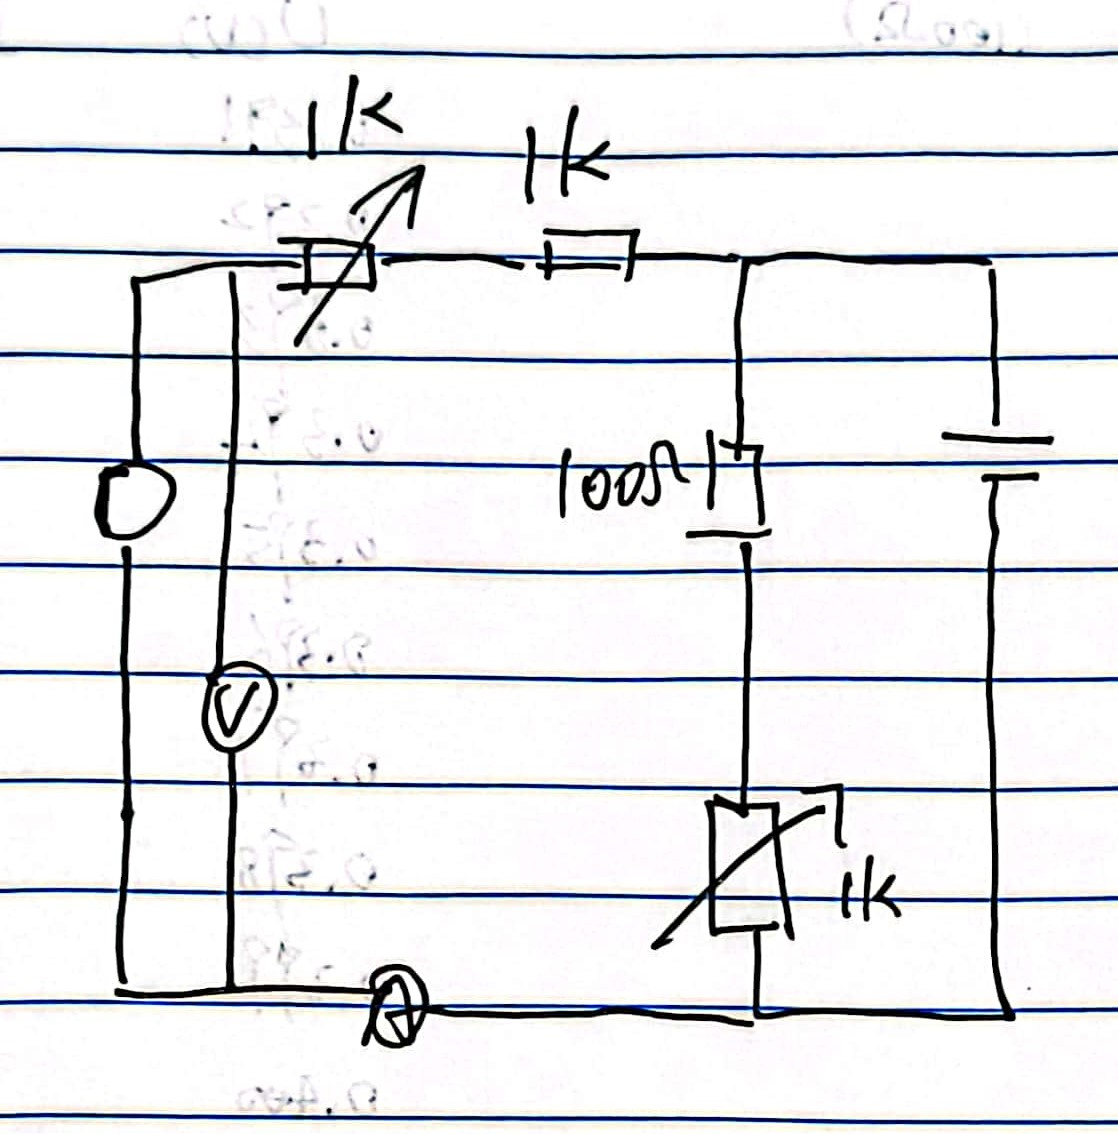
\includegraphics[width=0.46\textwidth]{fanxiangdianlu.jpg}
      \caption{二极管反向连通电路示意图}\label{fanxiangdianlu}
    \end{minipage}
  \end{figure}

  \(1\) 先使用数字多用表判断二极管的正负极。具体操作如下\\
  将数字多用表调节到二极管挡位,红黑表笔分别链接二极管的两端,观察万用表的示数。\\
  交换红黑表笔,在观察示数。\\
  若显示为0.7V左右电压,则表示红表笔一端为二极管的正极,另一端为负极。\\
  若反向链接,则显示为短路状态。\\
  若正反两个方向测得的结果一致,则表明该二极管已损坏。

  \(2\) 按照图\ref{zhengxiangdianlu}连接电路,将普通二极管连入伏安特性测量电路中。链接的时候注意
        正负极链接电源是否正确。调节电压,从0开始缓慢增加,观察电流。其中电流不要超过20mA,以免烧坏二极管。
        实验中需要测试15组数据。

  \(3\) 在作图纸上绘制正向伏安特性曲线。

  \(4\) 补充:最终实验没有测试反向击穿电压的原因是因为普通的二极管的反向击穿电压一般达到100V,远远超出了安全
        电压的范围,因此实验中不需要测量普通二极管的反向击穿电压。

  \subsection{测量稳压二极管的正向、反向伏安特性曲线}
  \(1\) 用数字多用表判断稳压二极管的正负极。
  
  \(2\) 按照图\ref{zhengxiangdianlu}连接电路,注意电流正向导通。测量15组数据

  \(3\) 按照图\ref{fanxiangdianlu}链接电路,注意电流反向导通。测试稳压二极管反向击穿电流特性。注意
        电流不要超过30mA,测量15组数据。测量反向击穿电压。

  \(4\) 在做图纸上作图得到伏安特性曲线。

  \subsection{测量发光二极管正向伏安特性曲线}
  \(1\) 参照普通二极管的实验步骤进行实验。测量15组数据。

  \(2\) 总共需要进行三个发光二极管的数据的测量和计算。

  \(3\) 计算发光二极管的峰值波长
\newpage


\section{实验原始数据}
\begin{figure}[H]
  \centering
  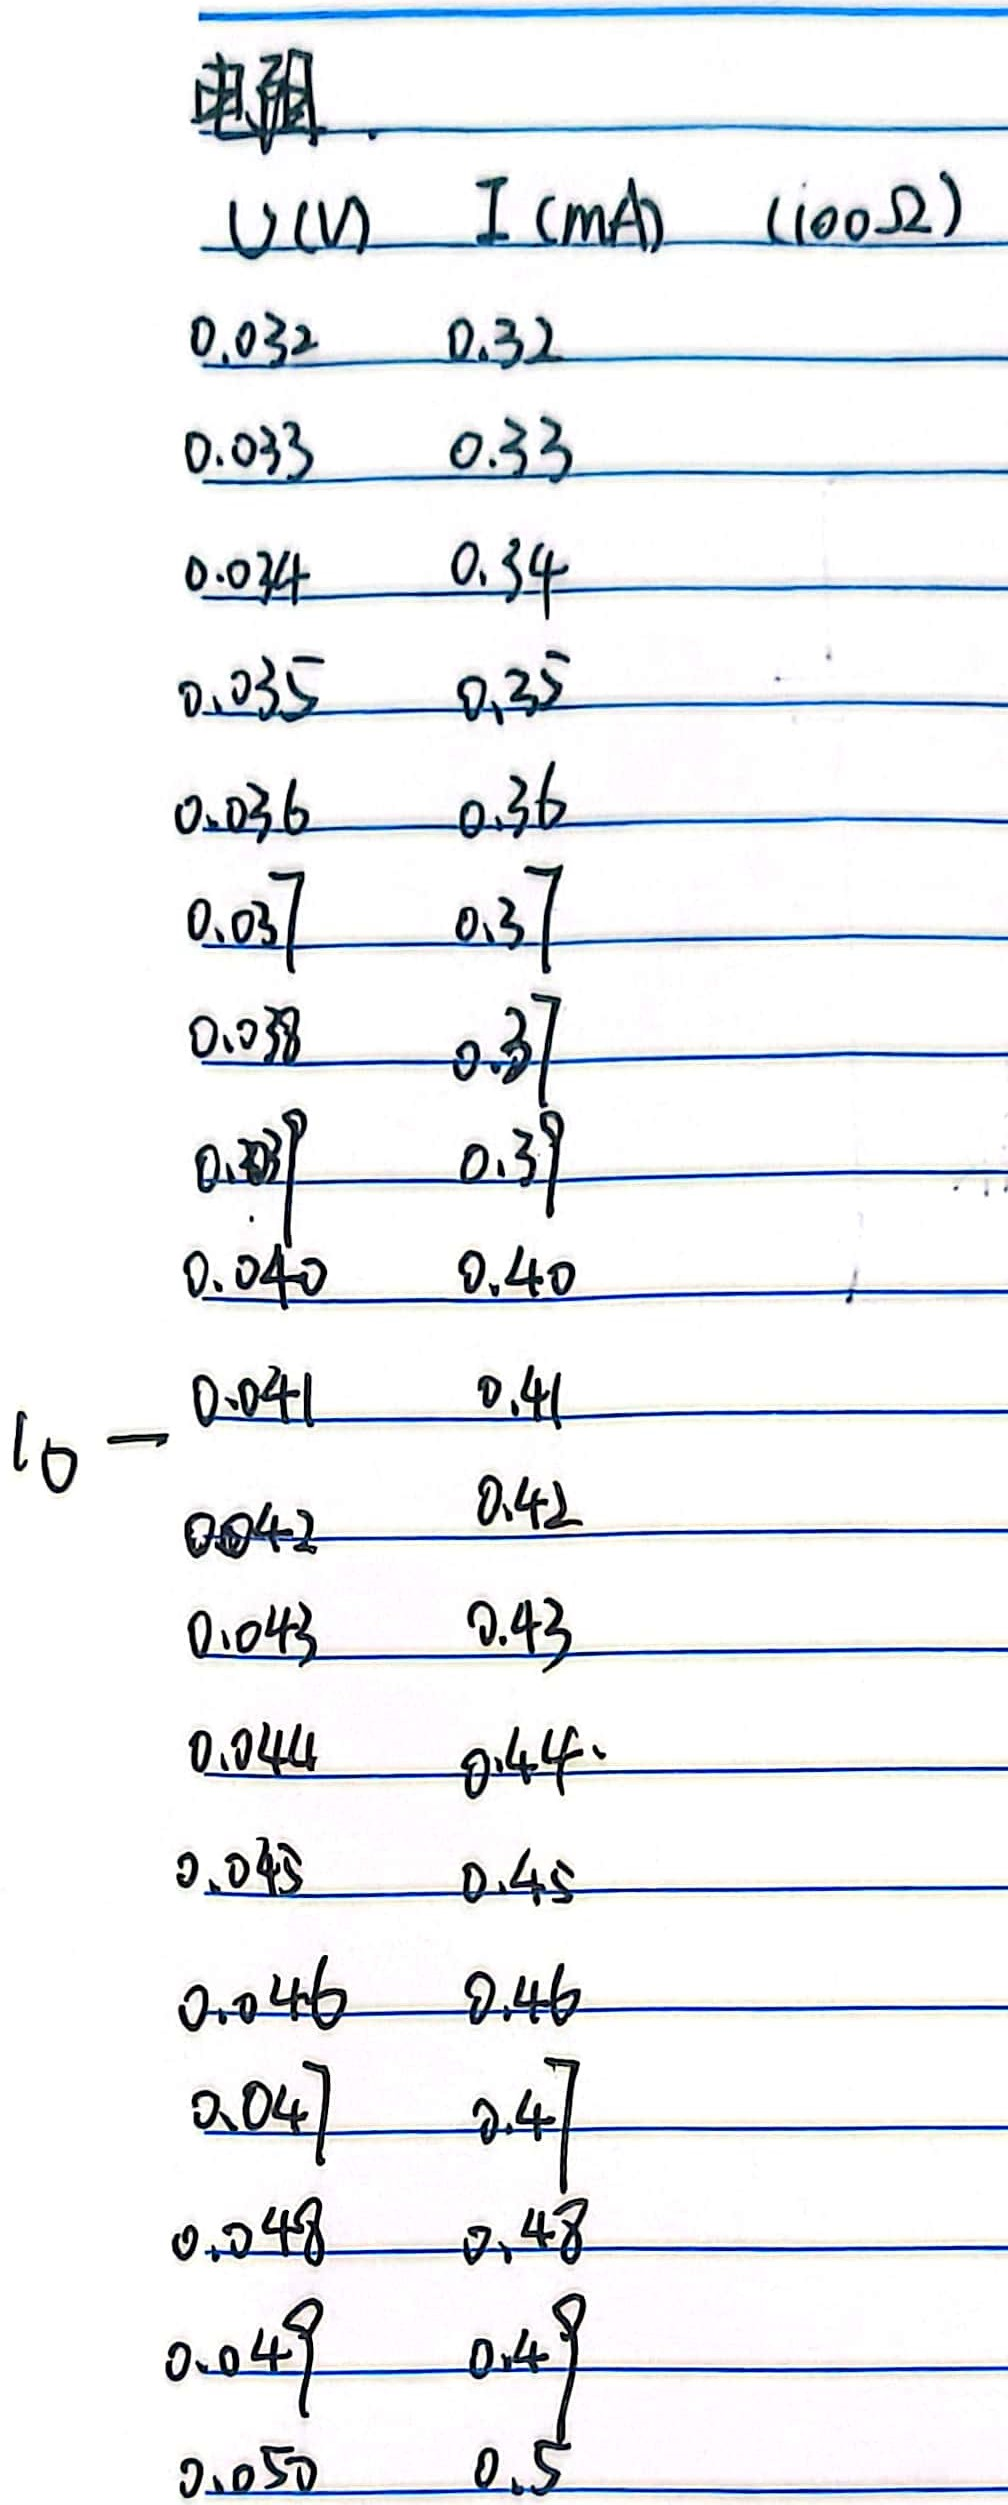
\includegraphics[width=0.9\textwidth,height=0.8\textheight]{dianzu.jpg}
  \caption{实验原始数据1}\label{dianzu}
\end{figure}
\newpage

\begin{figure}[H]
  \centering
  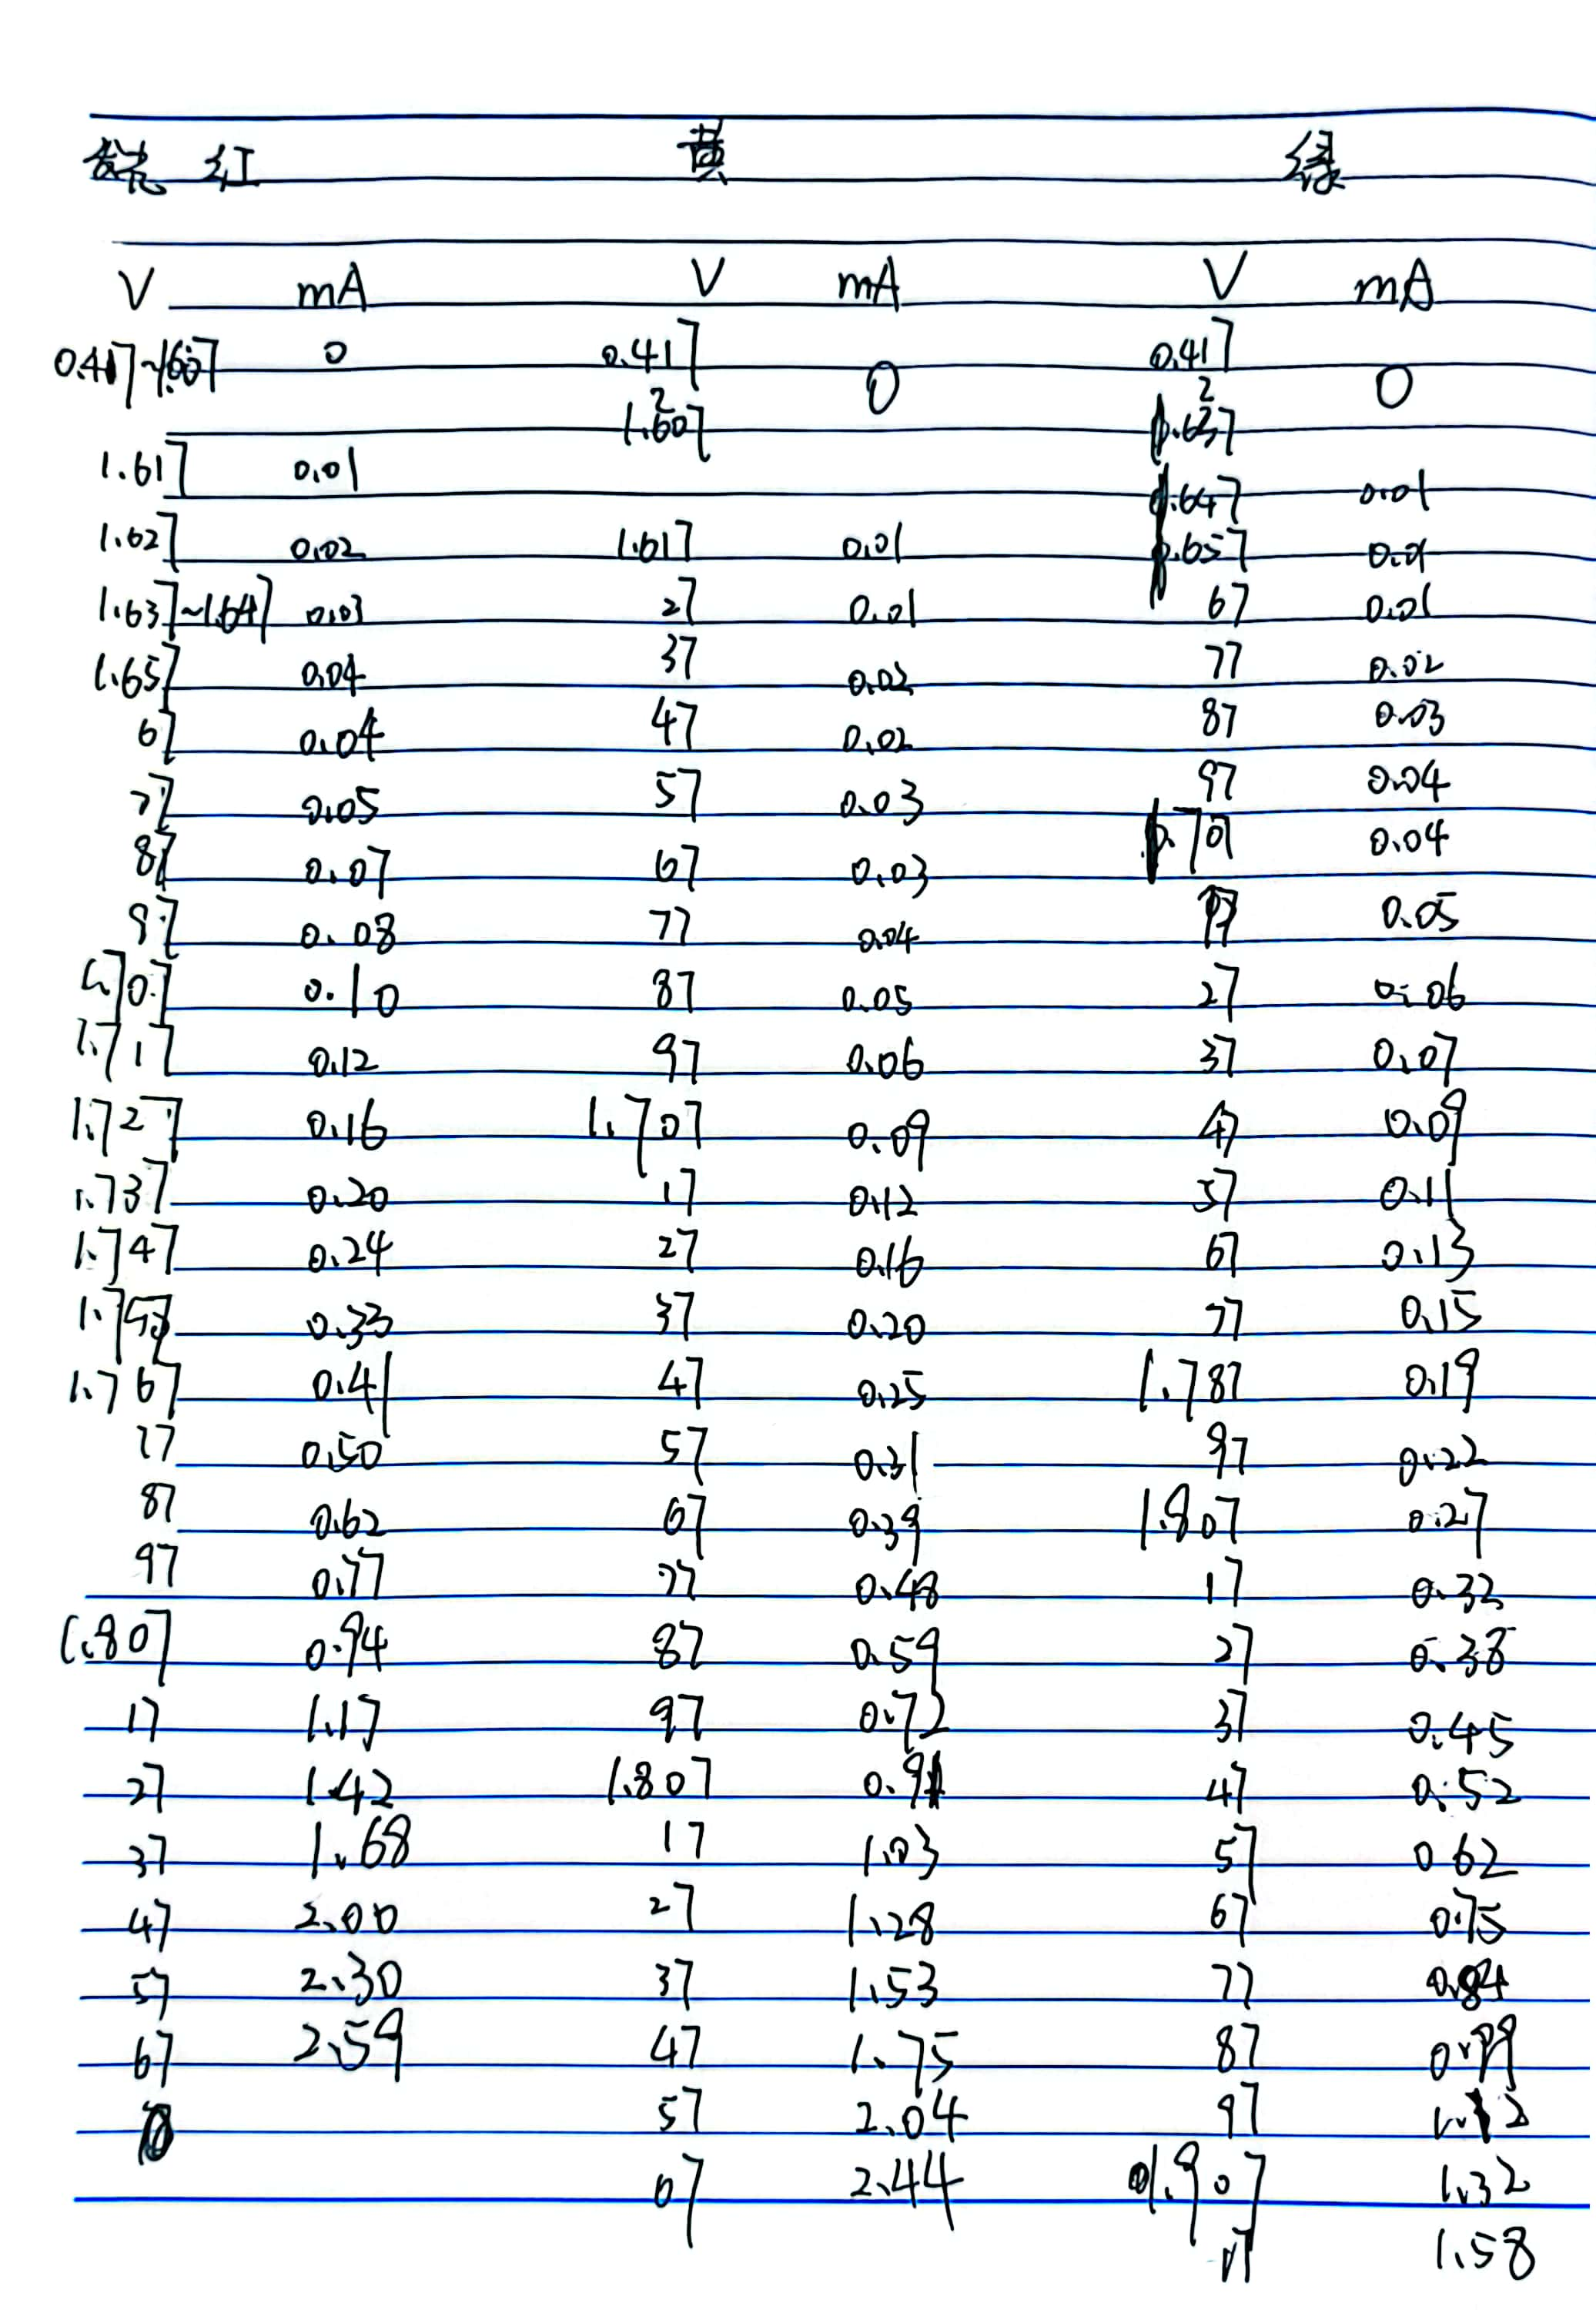
\includegraphics[width=1\textwidth,height=0.8\textheight]{LED1.jpg}
  \caption{实验原始数据2}\label{LED1}
\end{figure}
\newpage

\begin{figure}[H]
  \centering
  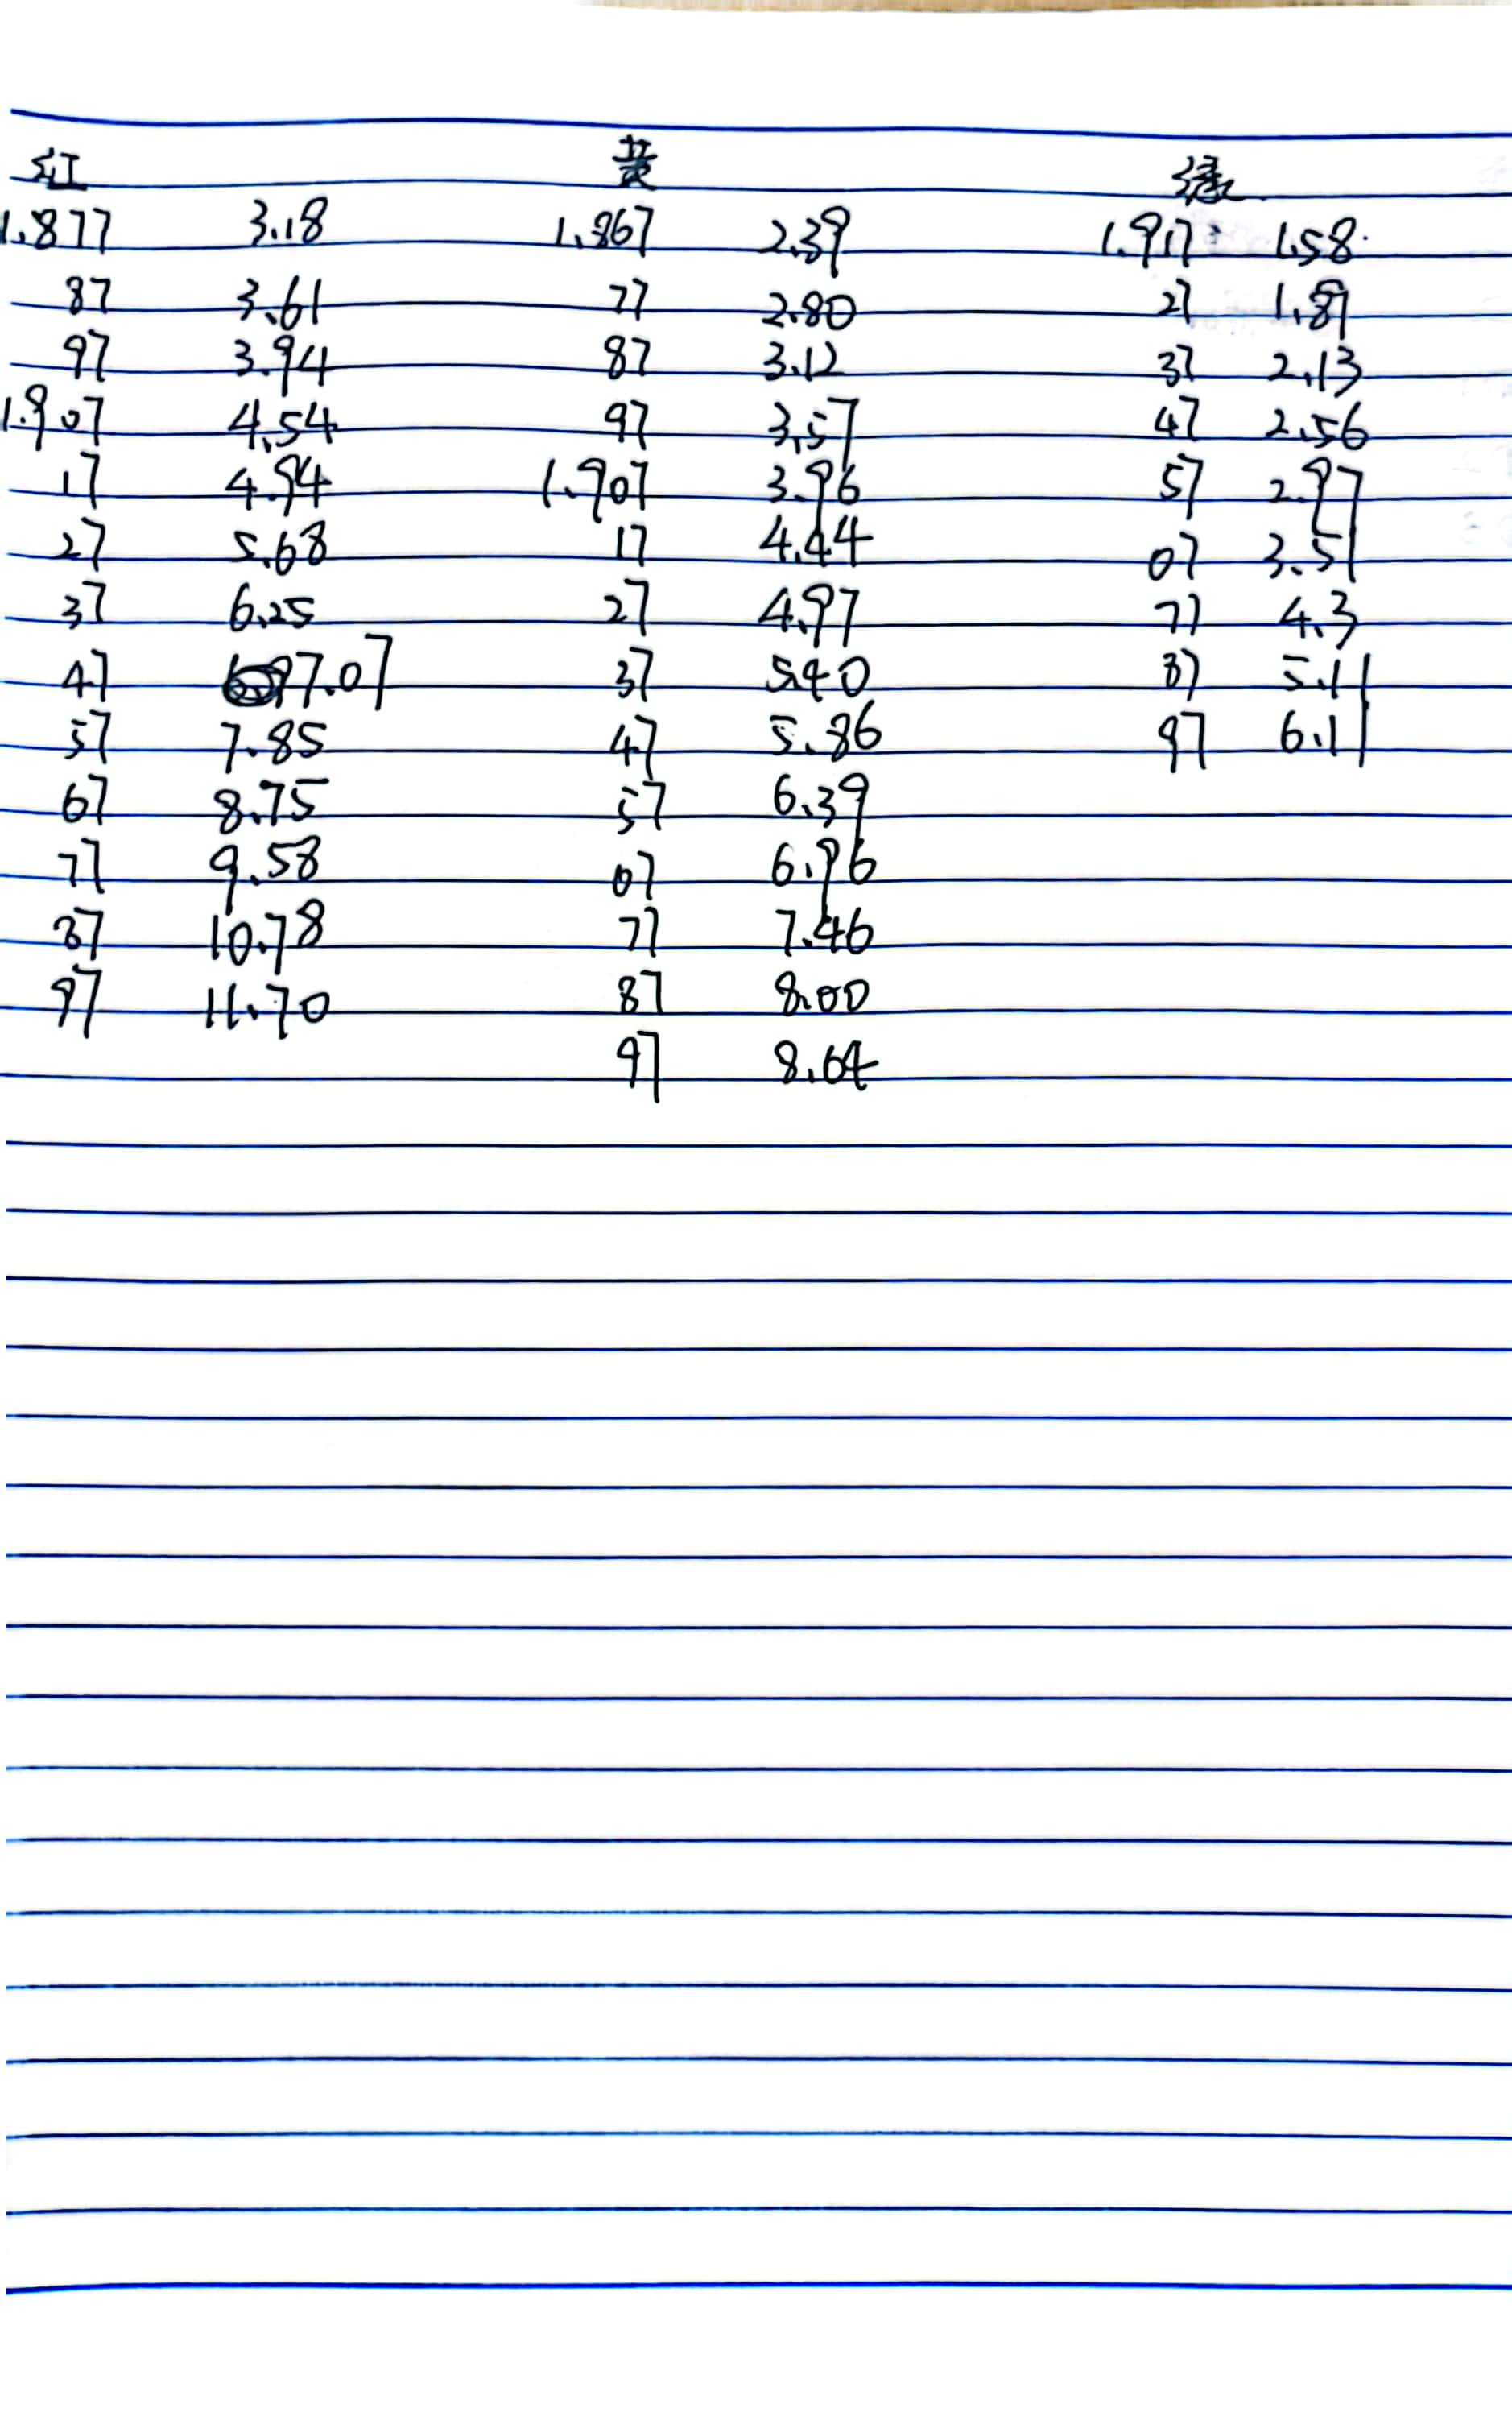
\includegraphics[width=1\textwidth,height=0.8\textheight]{LED2.jpg}
  \caption{实验原始数据3}\label{LED2}
\end{figure}
\newpage

\begin{figure}[H]
  \centering
  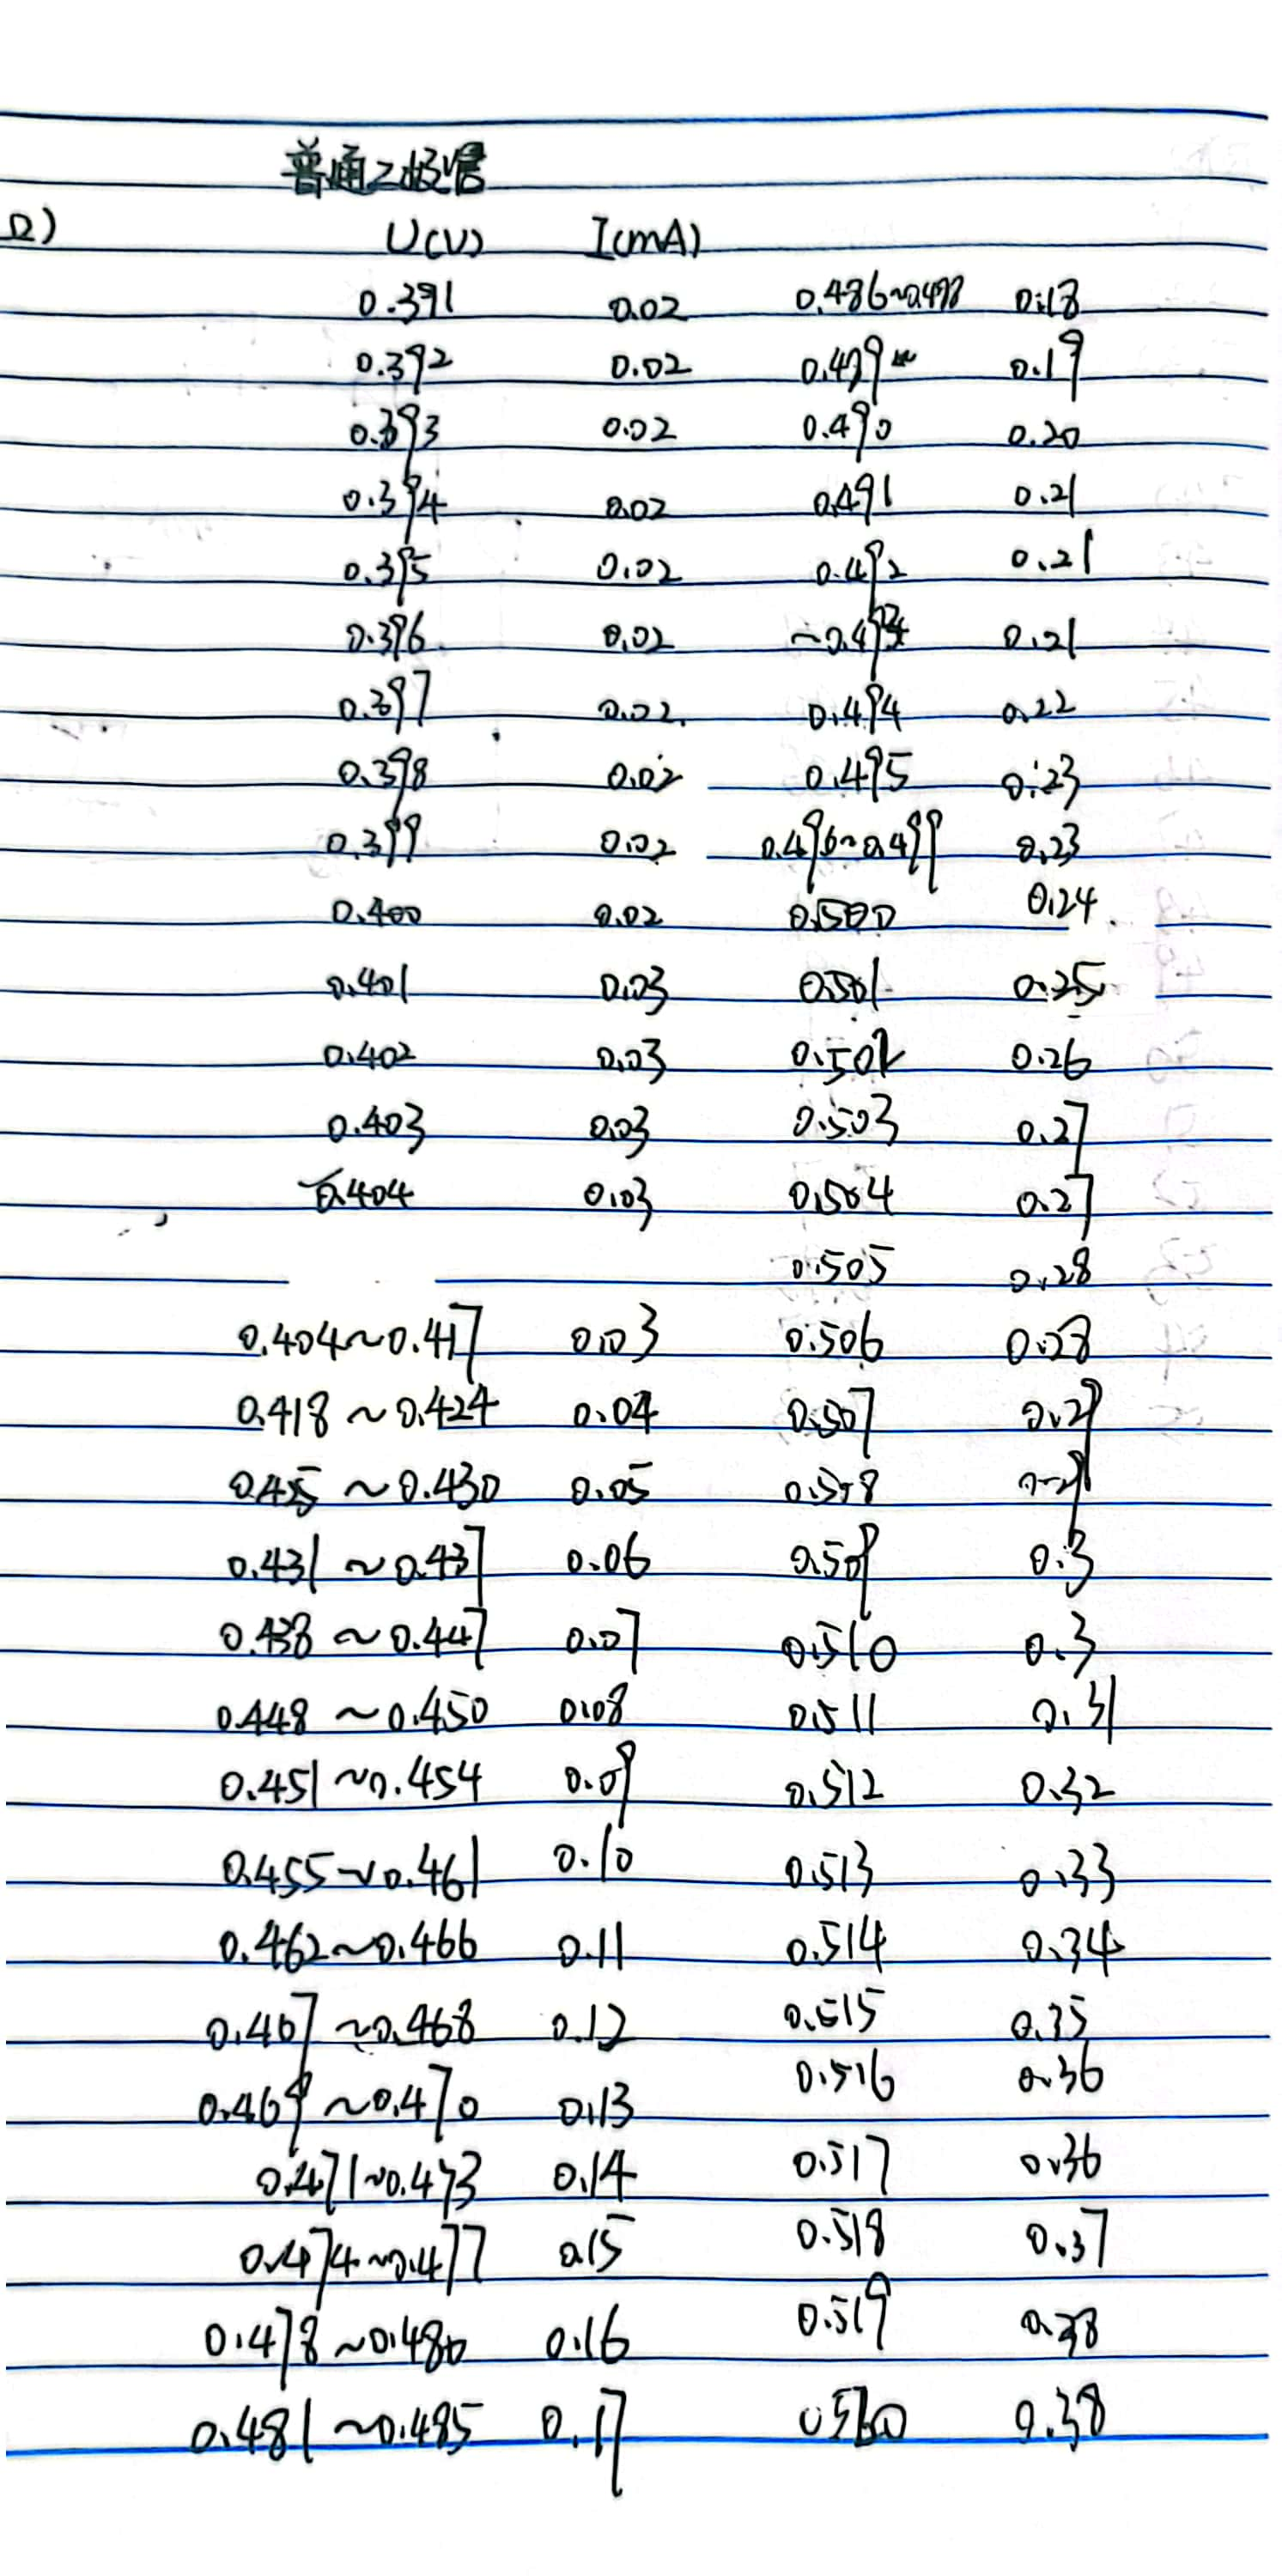
\includegraphics[width=1\textwidth,height=0.8\textheight]{putong1.jpg}
  \caption{实验原始数据4}\label{putong1}
\end{figure}
\newpage

\begin{figure}[H]
  \centering
  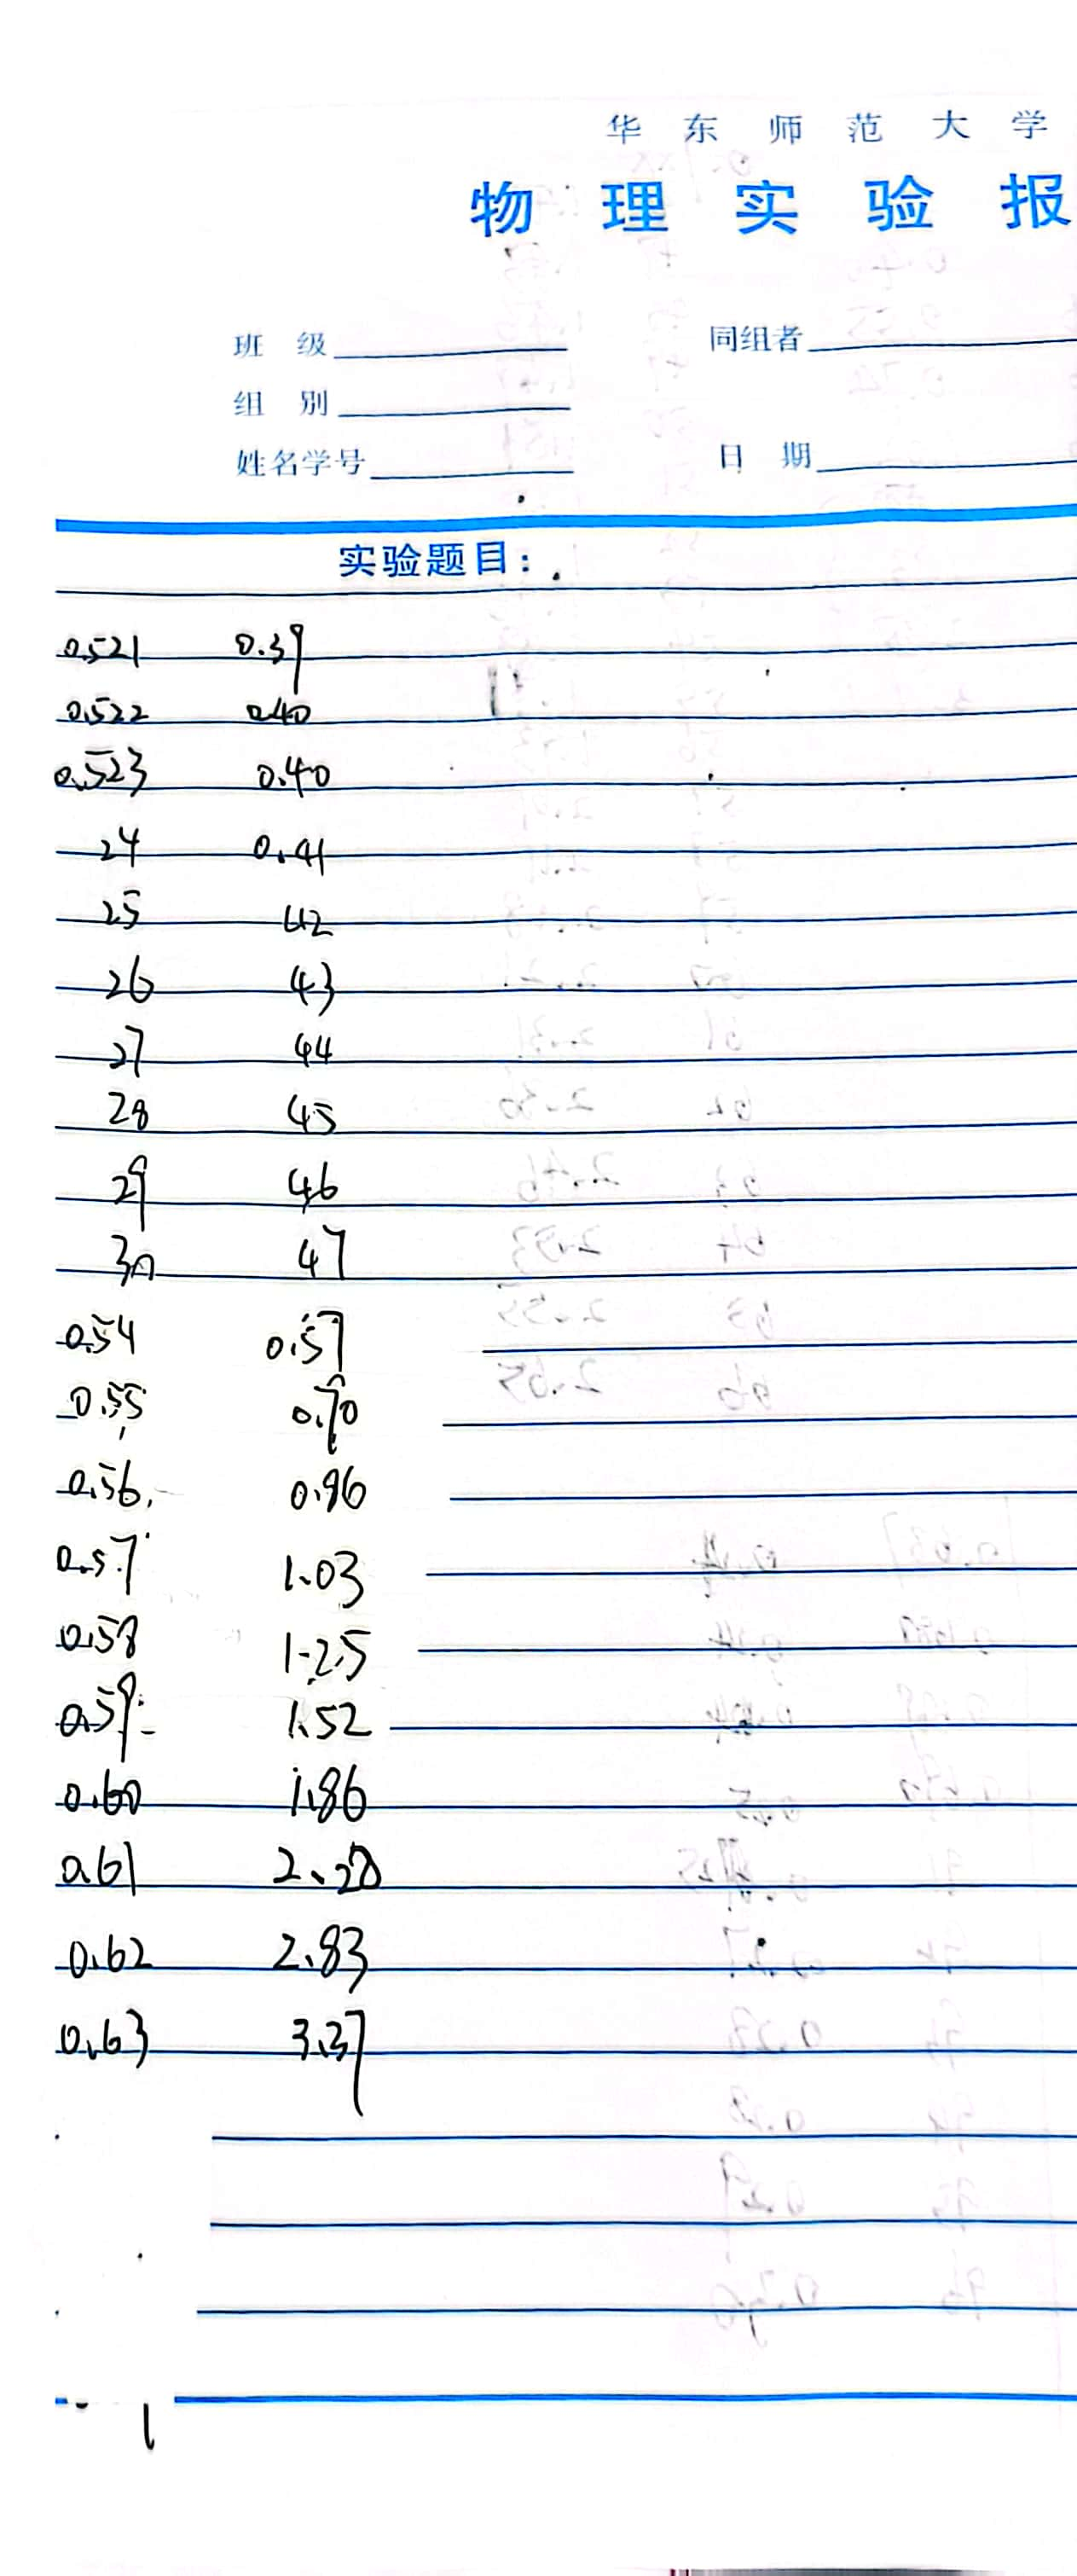
\includegraphics[width=1\textwidth,height=0.8\textheight]{putong2.jpg}
  \caption{实验原始数据5}\label{putong2}
\end{figure}
\newpage

\begin{figure}[H]
  \centering
  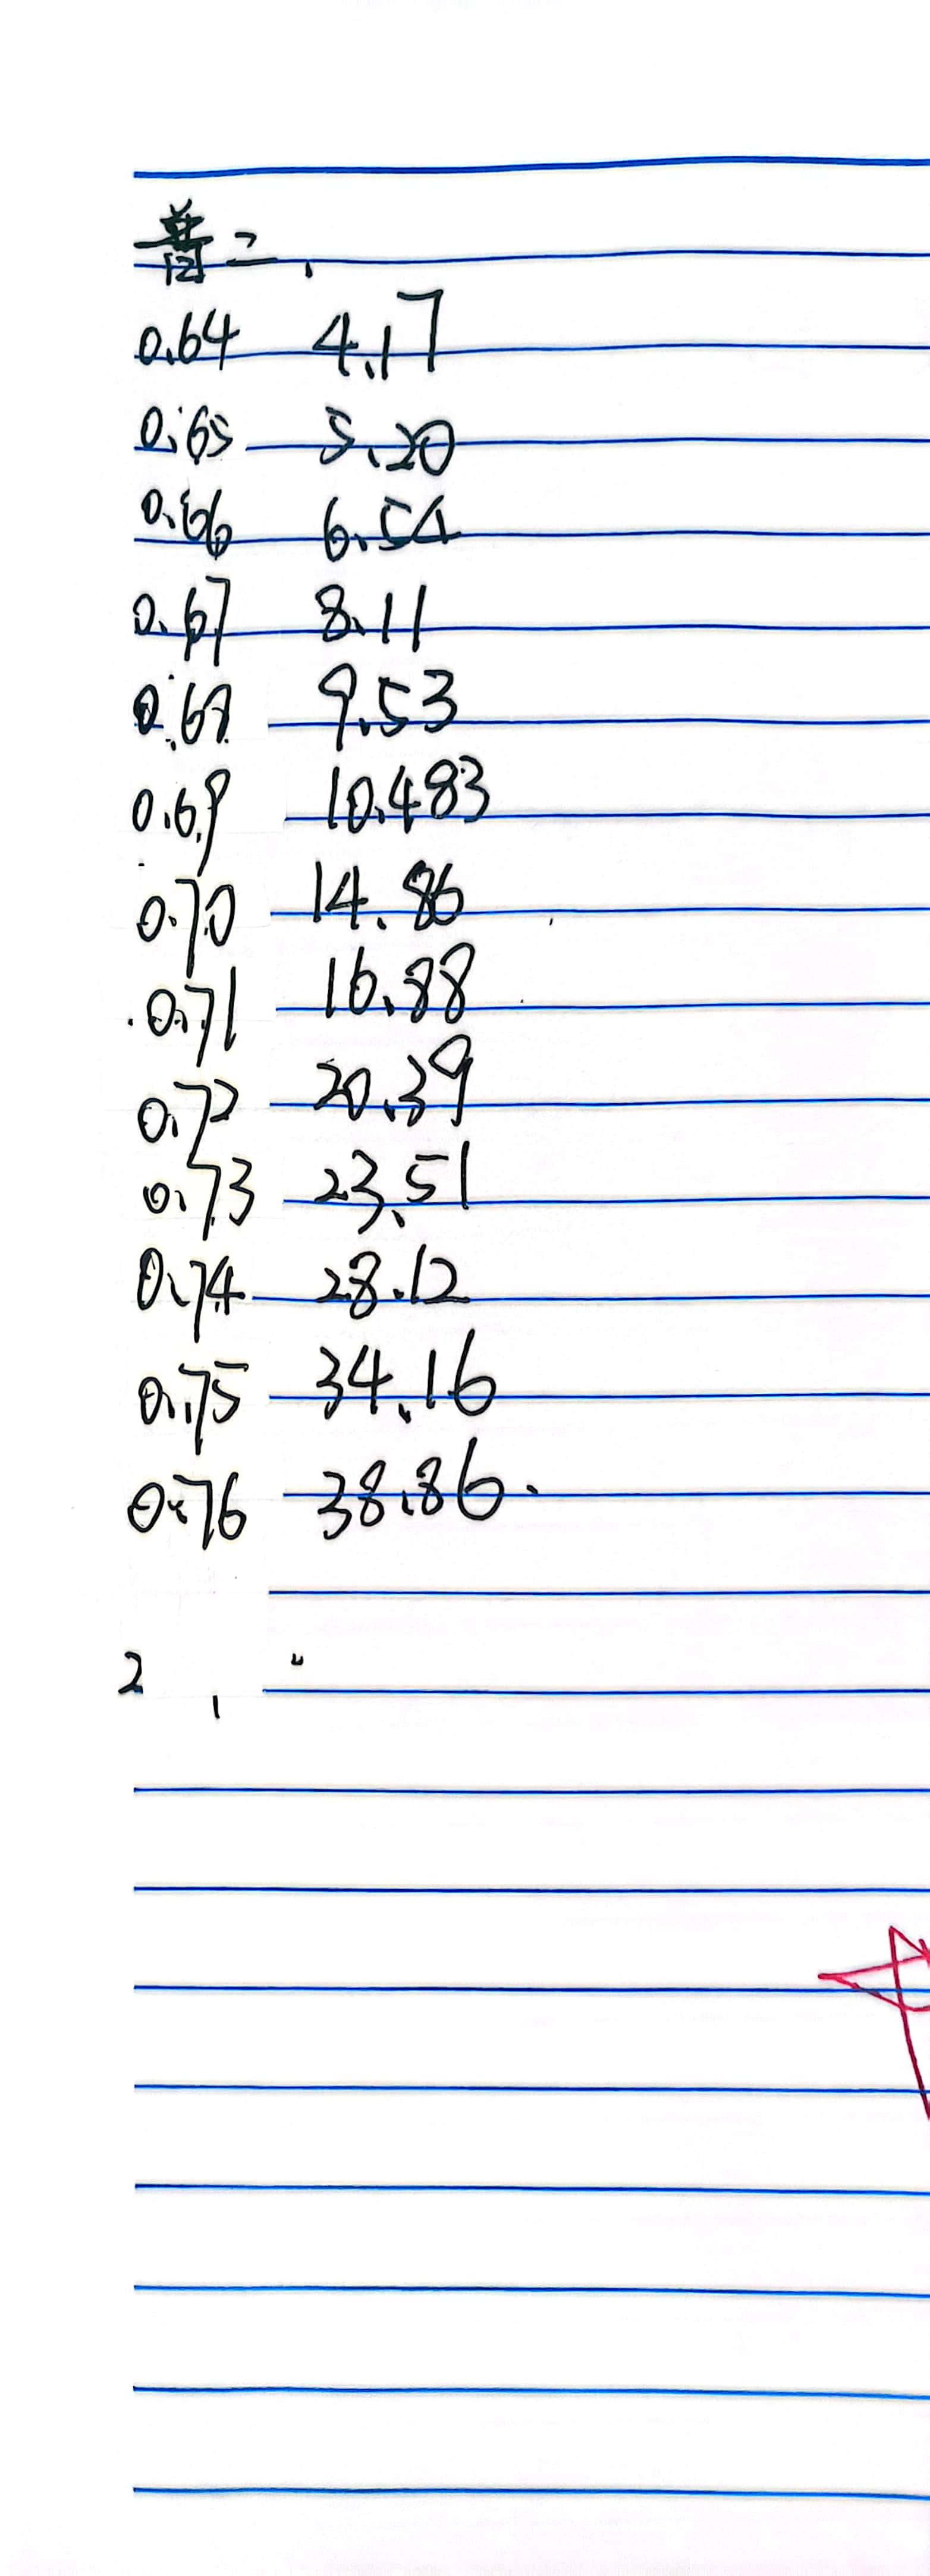
\includegraphics[width=1\textwidth,height=0.8\textheight]{putong3.jpg}
  \caption{实验原始数据6}\label{putong3}
\end{figure}
\newpage

\begin{figure}[H]
  \centering
  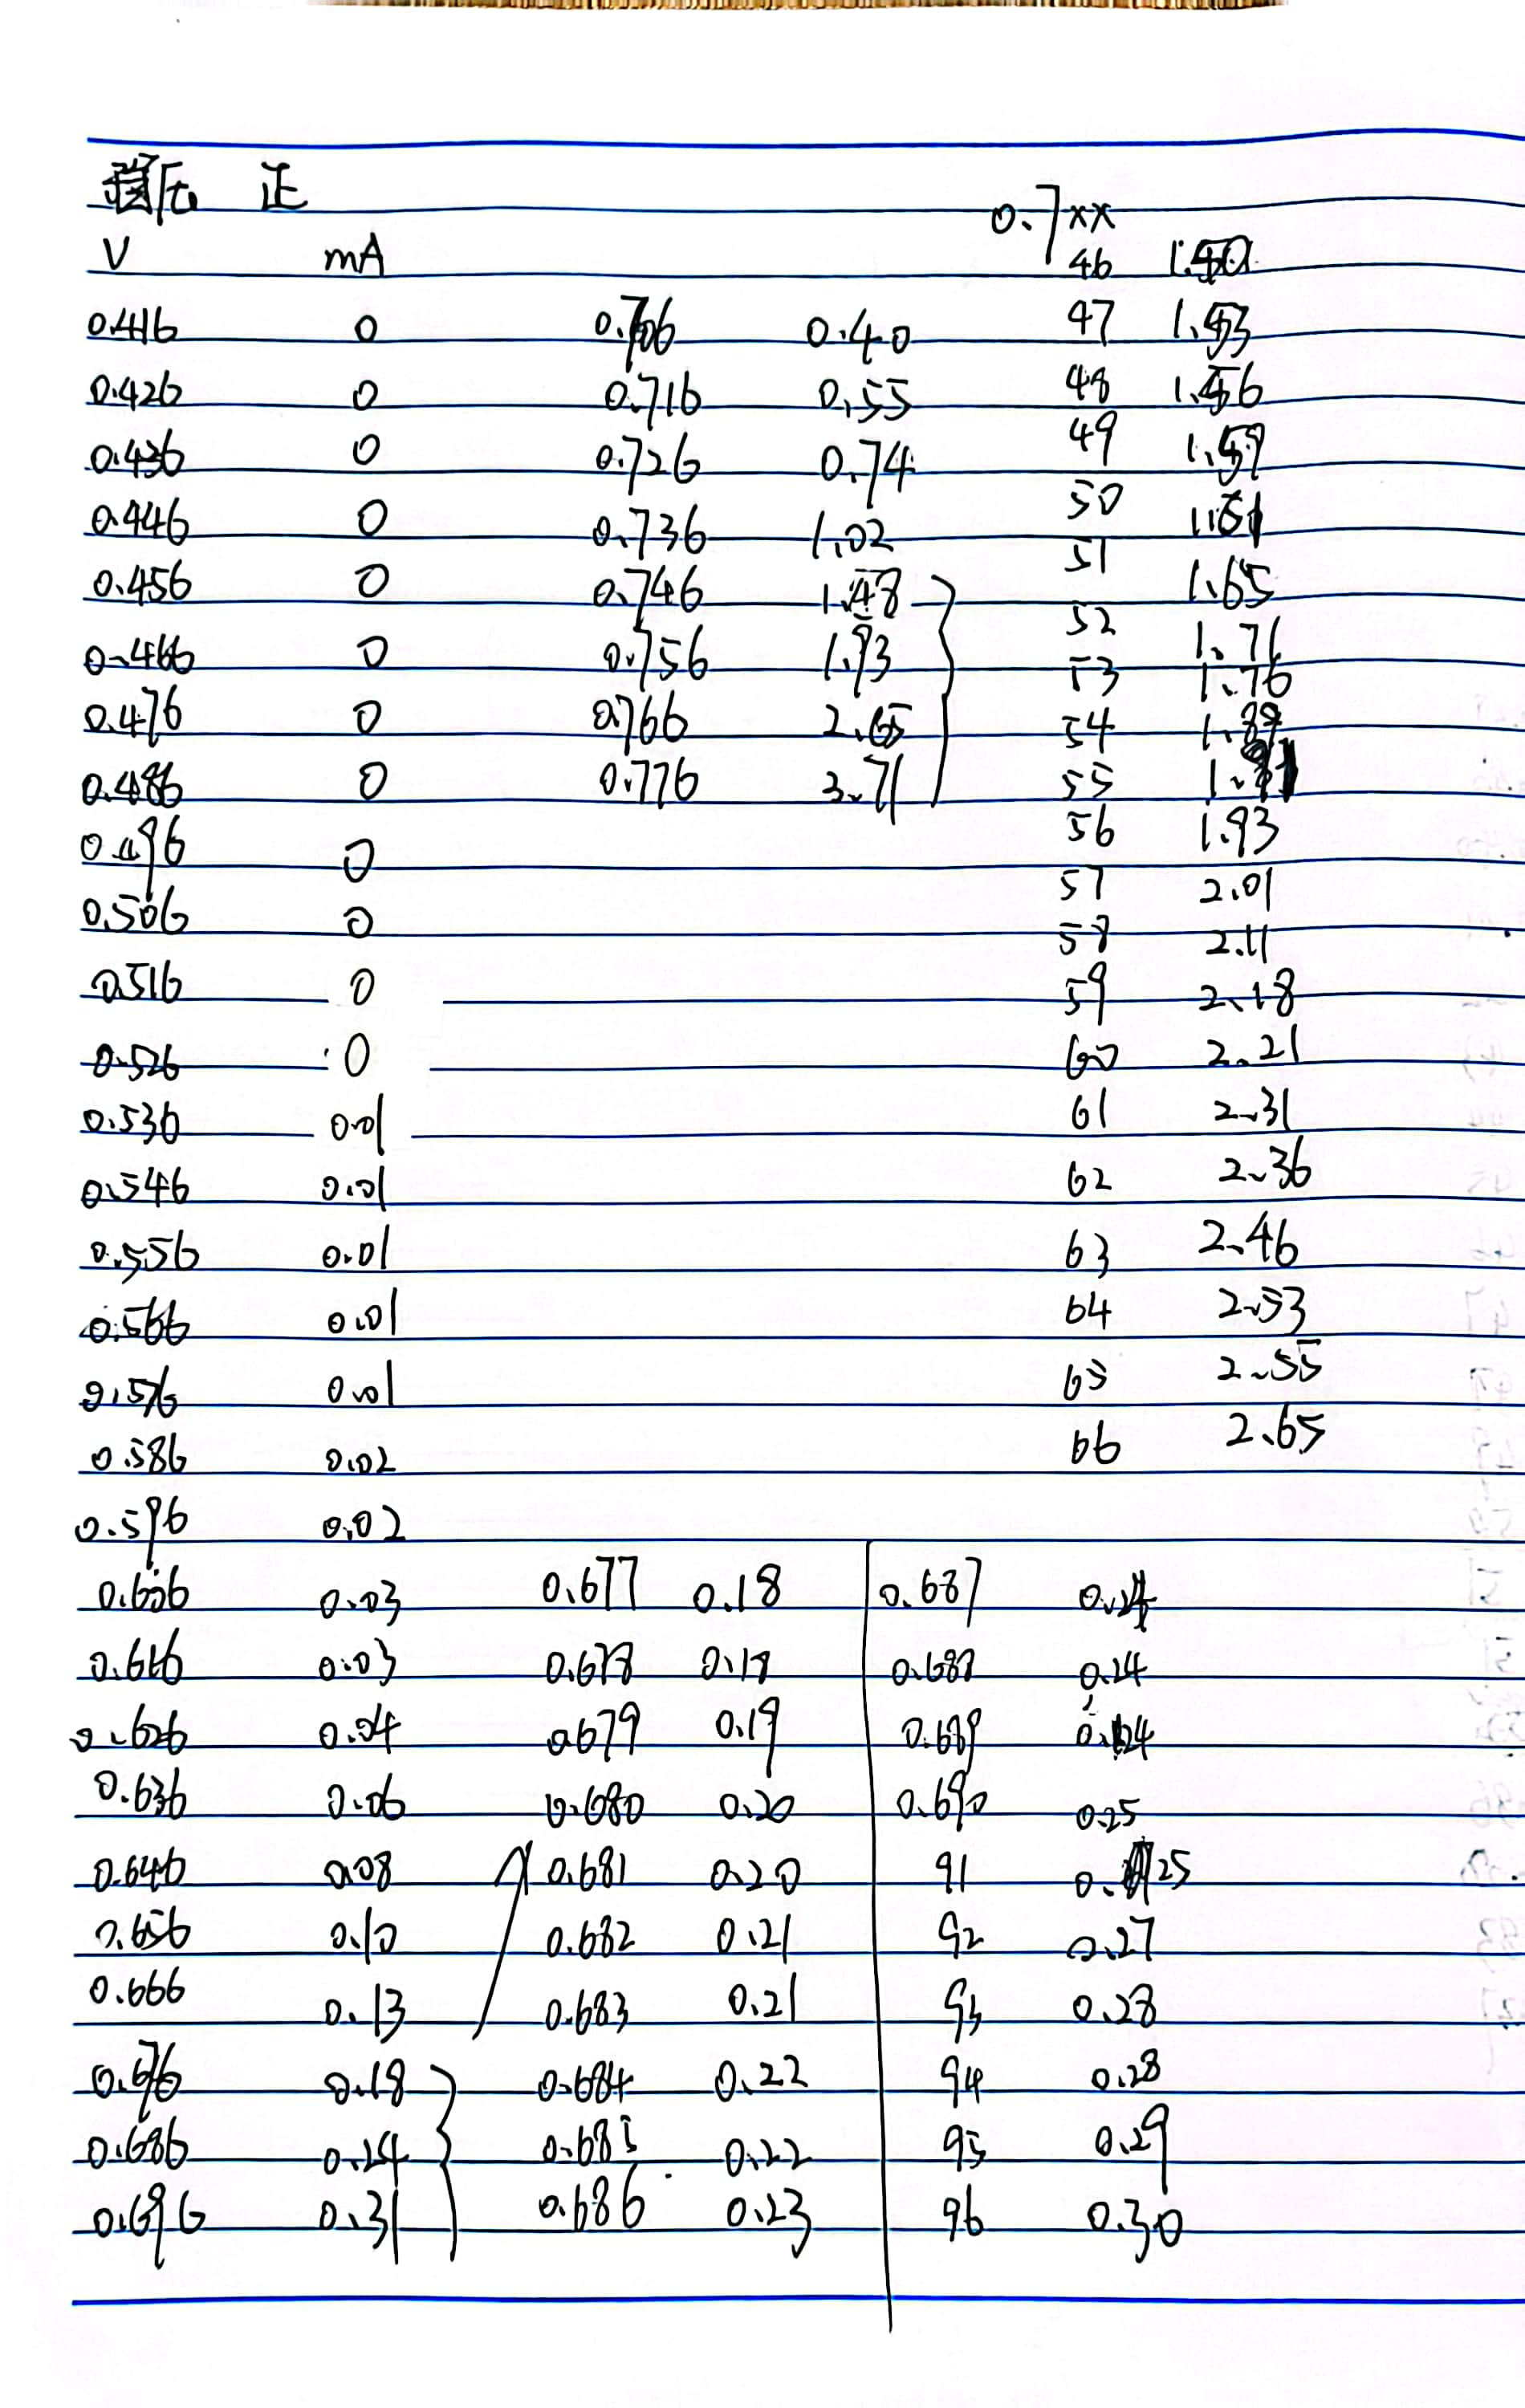
\includegraphics[width=1\textwidth,height=0.8\textheight]{wenyazhengxiang1.jpg}
  \caption{实验原始数据7}\label{wenyazhengxiang1}
\end{figure}
\newpage

\begin{figure}[H]
  \centering
  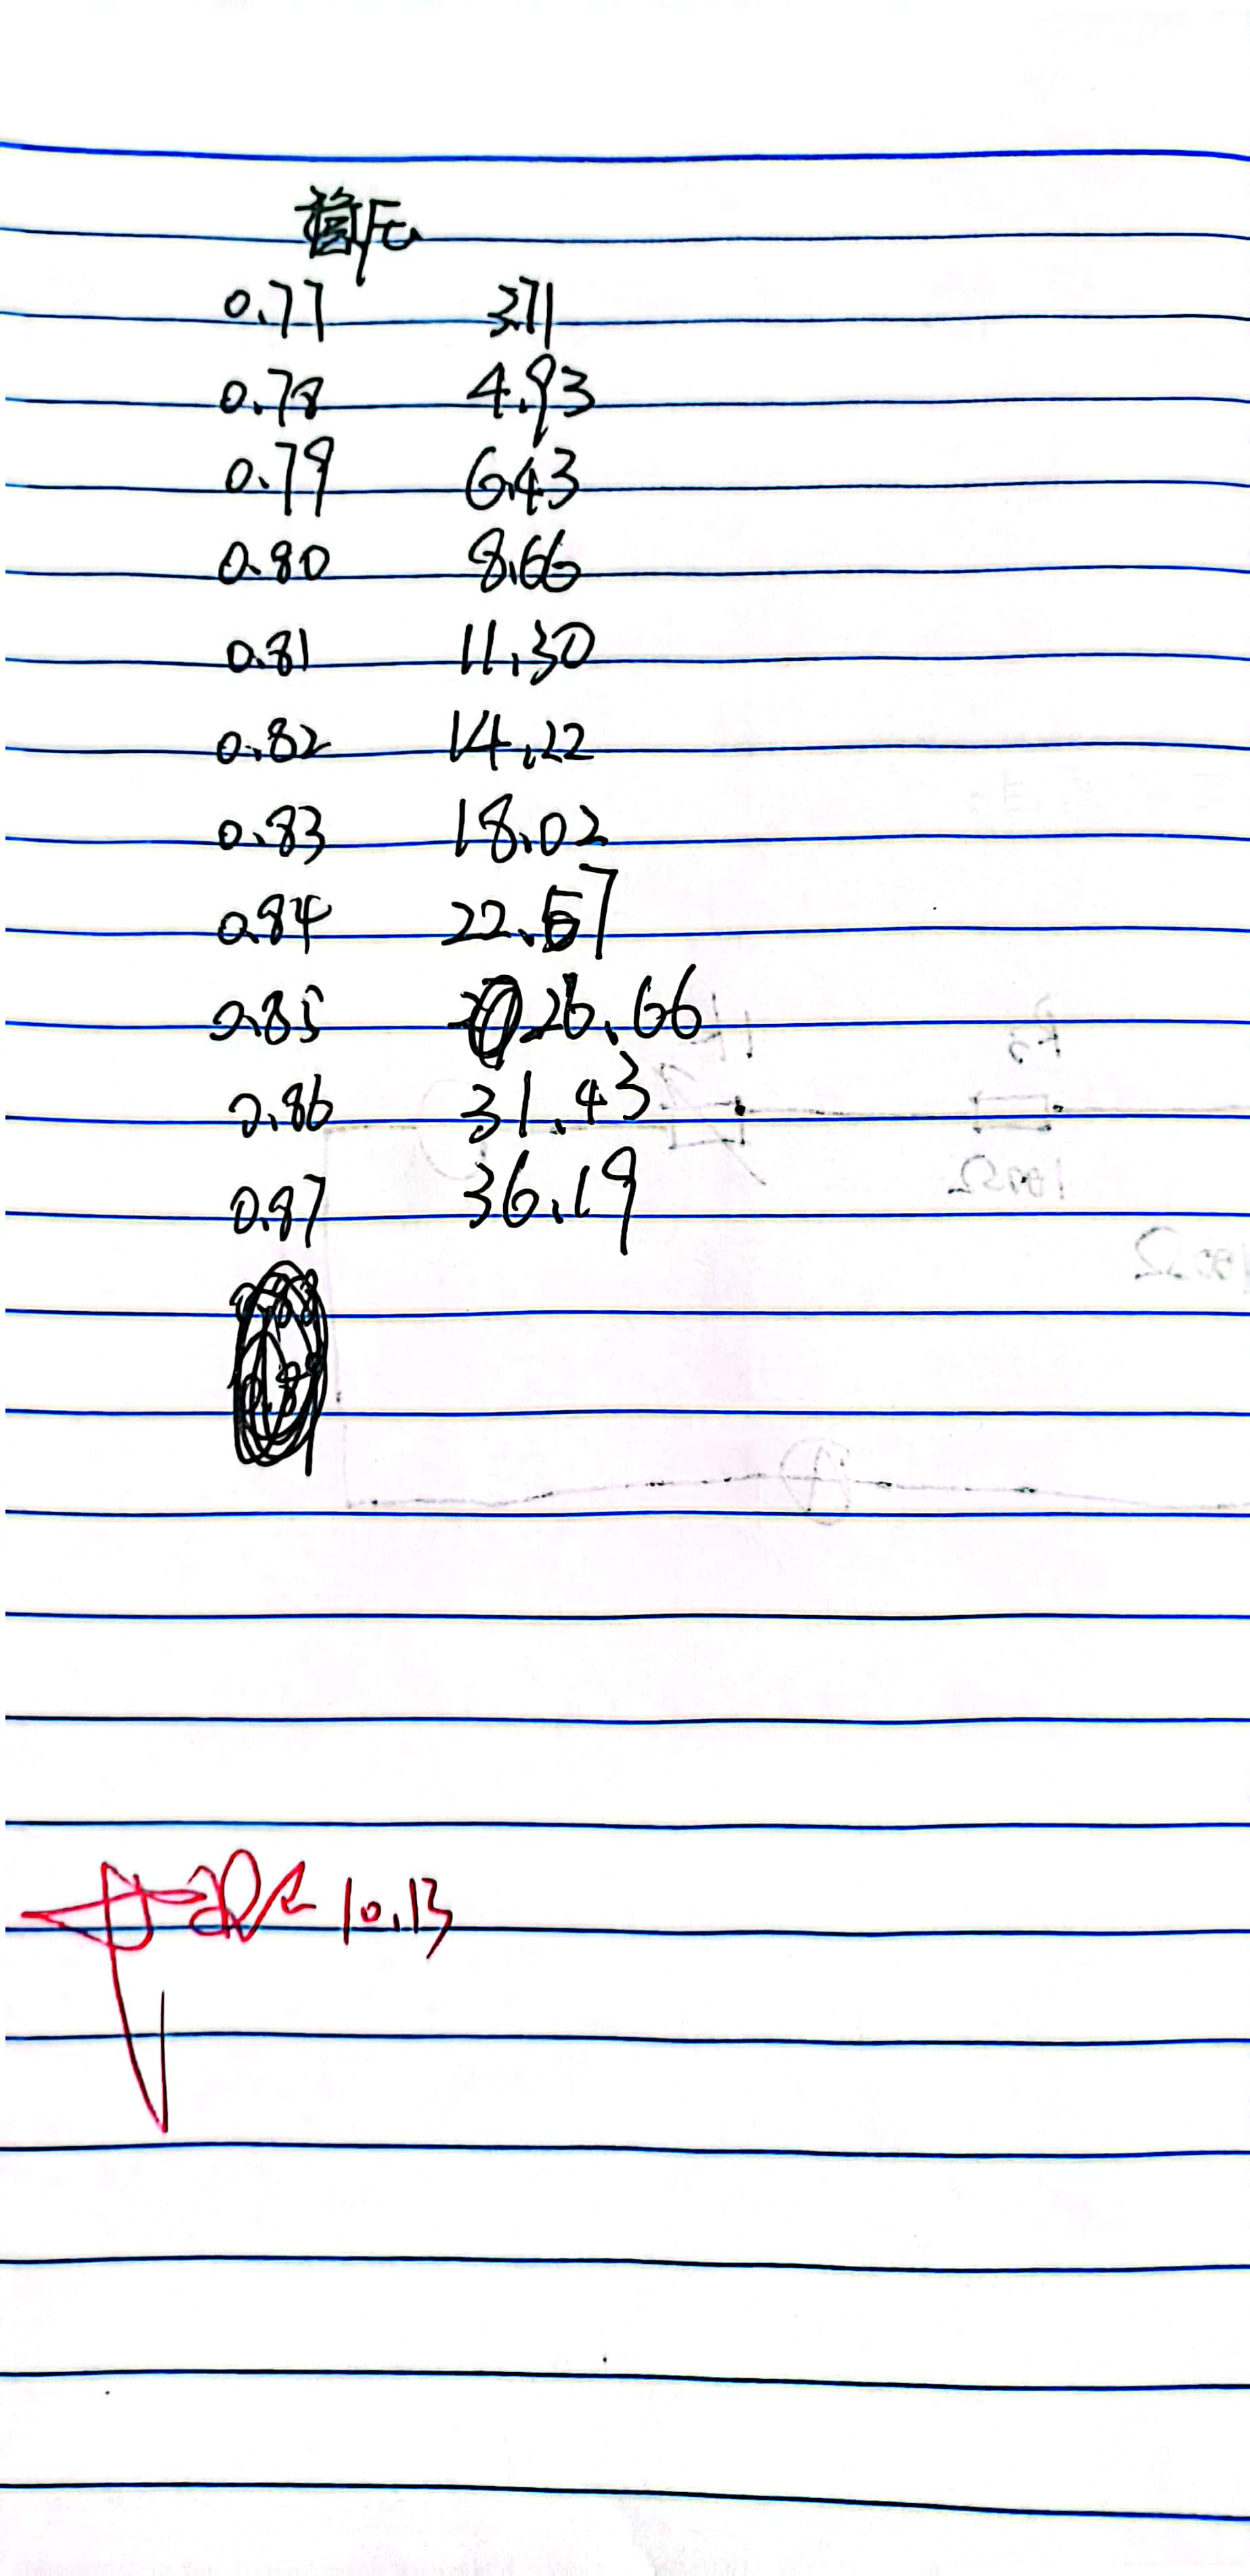
\includegraphics[width=1\textwidth,height=0.8\textheight]{wenyazhengxiang2.jpg}
  \caption{实验原始数据8}\label{wenyazhengxiang2}
\end{figure}
\newpage

\begin{figure}[H]
  \centering
  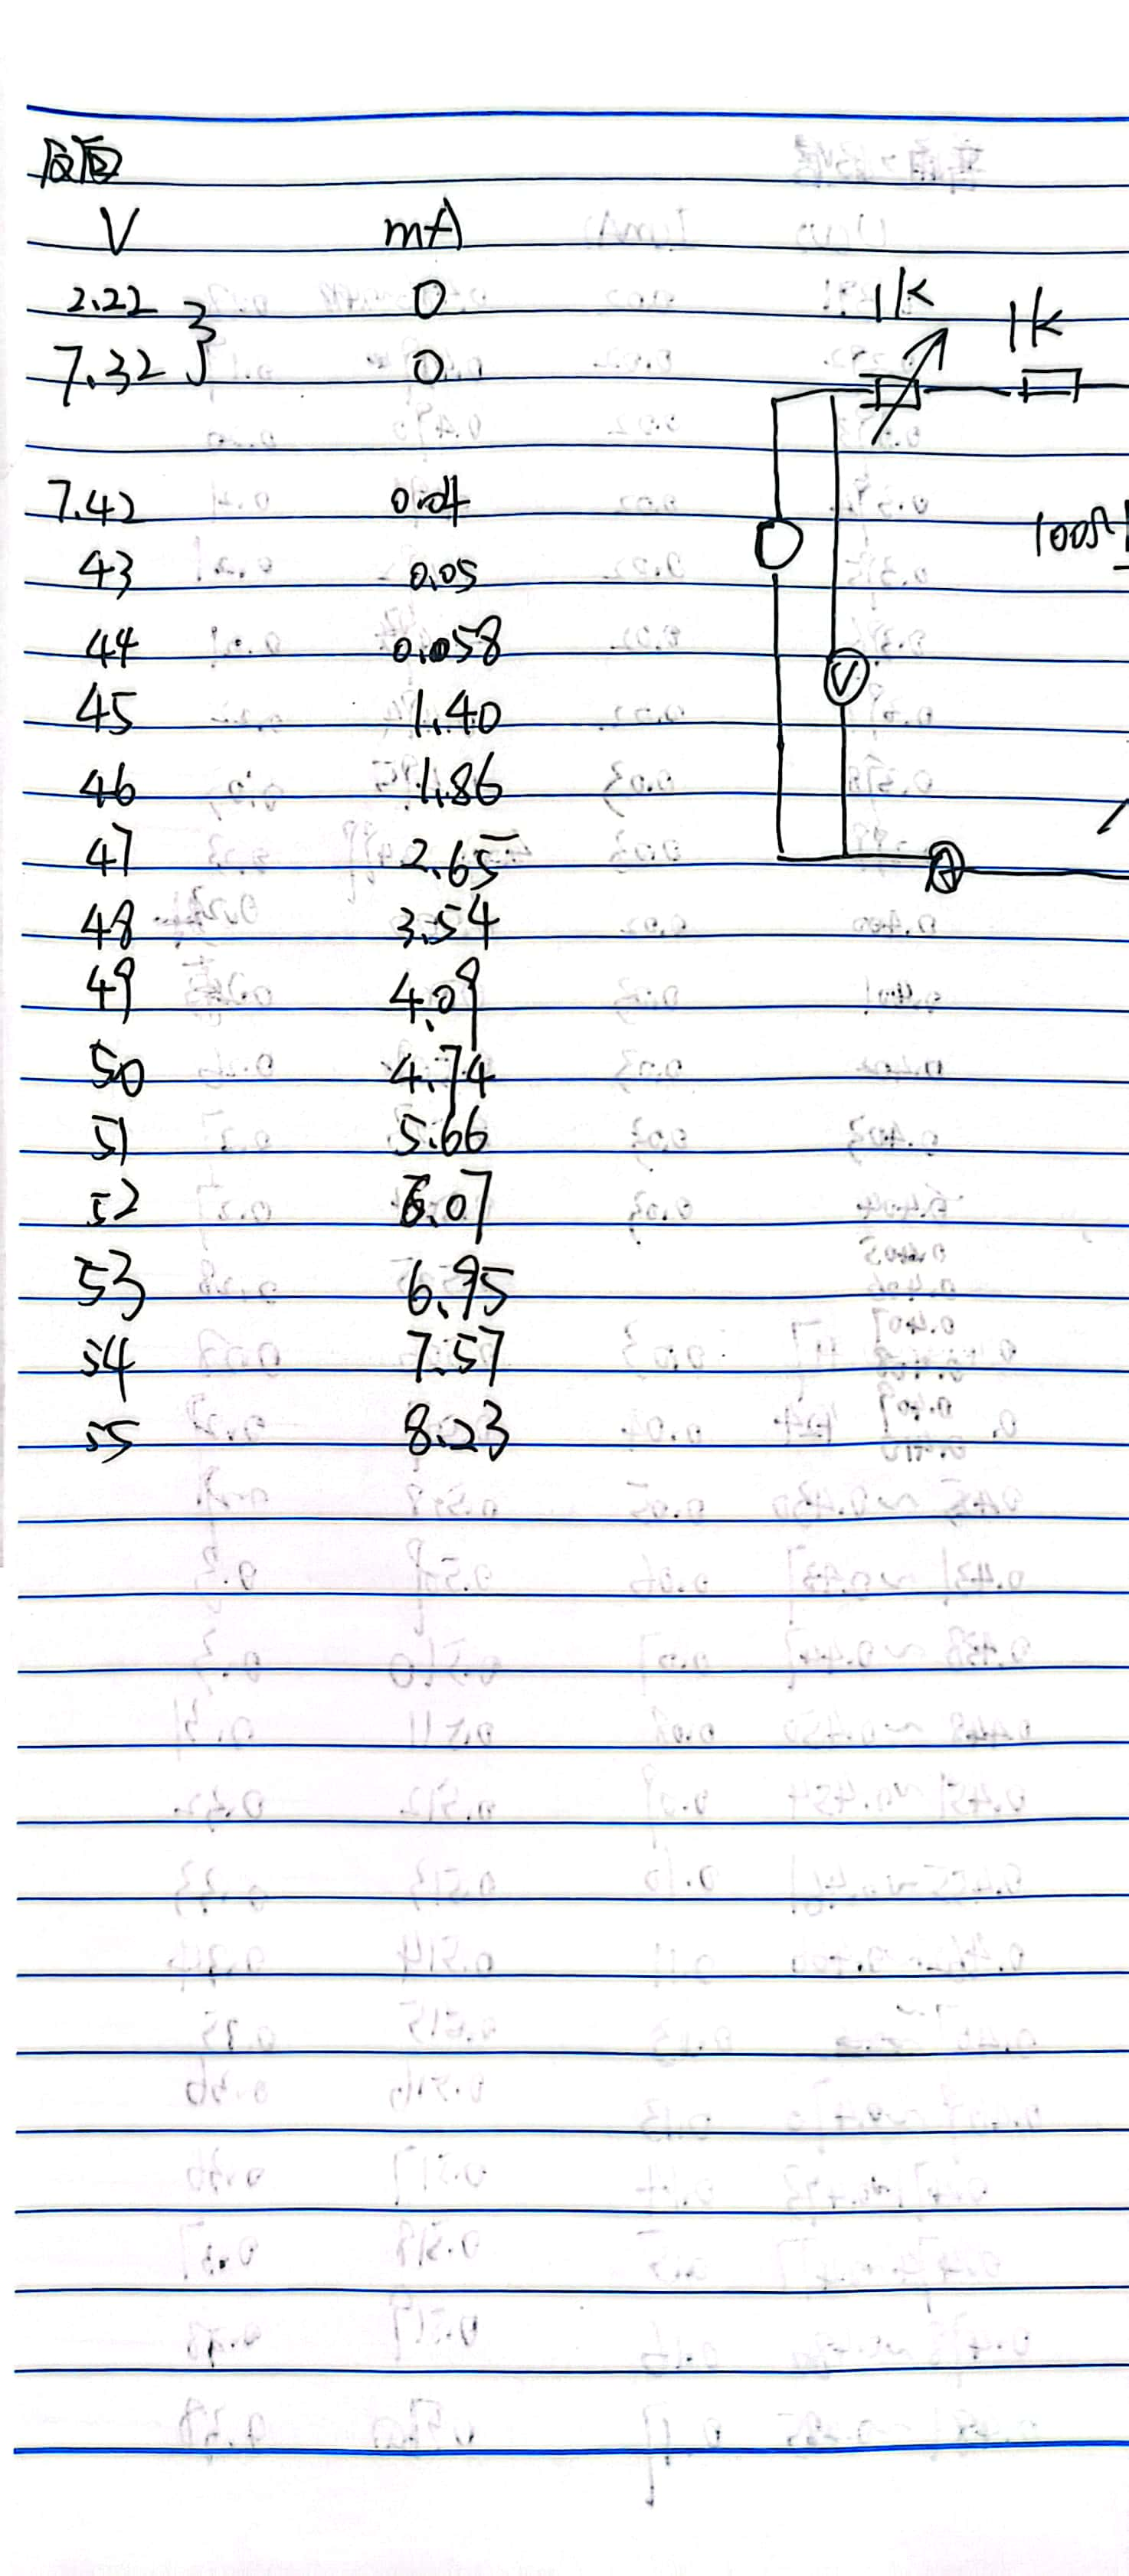
\includegraphics[width=1\textwidth,height=0.8\textheight]{wenyafanxiang.jpg}
  \caption{实验原始数据9}\label{wenyafanxiang}
\end{figure}
\newpage





% \section{实验数据处理}
% 弹簧质量显示如表\ref{tanhuangzhiliang}
% \begin{table}[h]
%   \centering   
%   \caption{弹簧弹性系数及该系数弹簧的质量对应关系示意图}\label{tanhuangzhiliang}
%   \begin{tabular}{| l || l |}
%       \hline
%       弹性系数的弹簧 & 弹簧质量(克)\\
%       \hline
%       0.961 & 13.61 \\
%       \hline
%       5.499 & 20.28 \\
%       \hline
%       8.828 & 17.62 \\
%       \hline
%       2.510 & 17.06 \\
%       \hline                       
%   \end{tabular}
% \end{table}
%   \subsection{验证位移方程}
%   \begin{figure}[b]
%     \centering
%     \begin{minipage}[b]{0.48\textwidth}
%       \centering
%       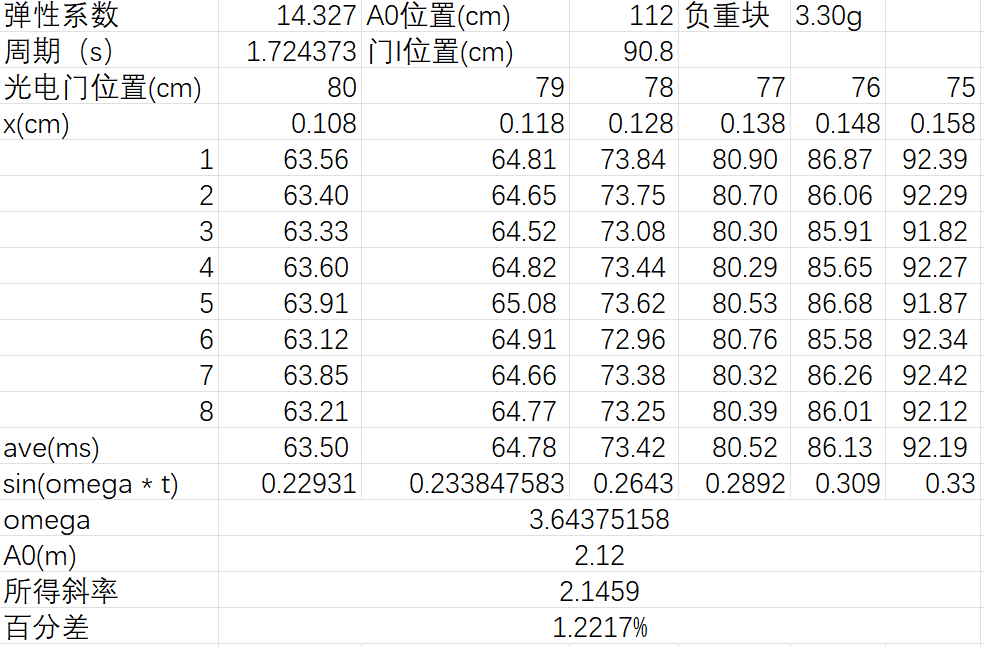
\includegraphics[width=0.46\textwidth]{yanzhengweiyifangchengshujv.png}
%       \caption{验证位移方程数据}\label{yanzhengweiyifangchengshujv}
%     \end{minipage}
%     \begin{minipage}[b]{0.48\textwidth}
%       \centering
%       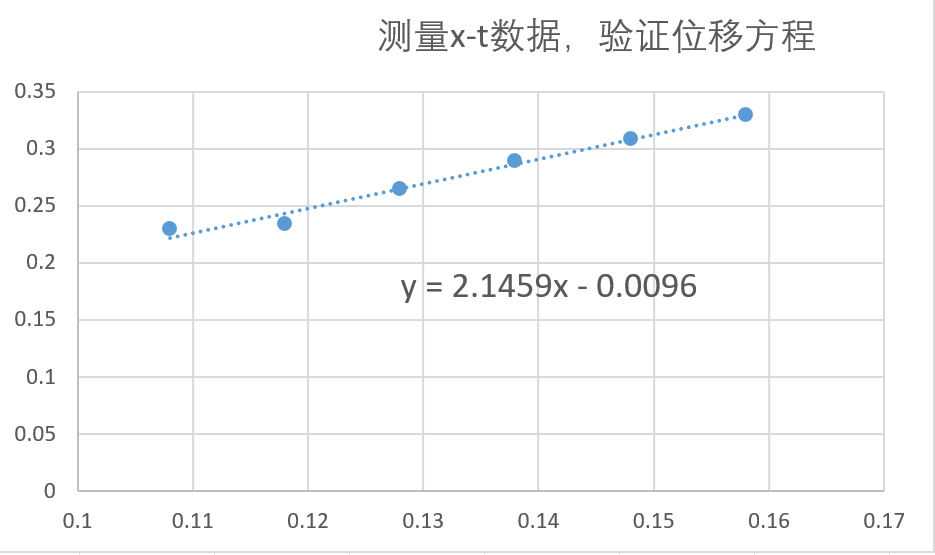
\includegraphics[width=0.46\textwidth]{yanzhengweiyifangchengzuotu.png}
%       \caption{验证位移方程作图法}\label{yanzhengweiyifangchengzuotu}
%     \end{minipage}
%   \end{figure}

%   实验数据处理如图\ref{yanzhengweiyifangchengshujv},其中计算可得实验理论$A_{0}=2.12dm$,而实验所得
%   斜率,即实际测量的实际$A_{0}=2.1459dm$,两者的相差程度,即百分差为$1.2217\%$。可以证明位移方程
%   $x=A\sin \left( \omega t + {\varphi}_{0} \right) \mbox{在}{\varphi}_{0} = 0 $时成立。

%   实验中的误差可能来源于

%   1、每次释放位置不能保证完全相同

%   2、光电门传感器精度限制,以及挡光板的宽度

%   3、实验中气垫滑轨不能保证完全水平,出现倾斜

%   \subsection{验证振动周期与初始状态无关}
%   \begin{figure}[t]
%     \centering
%     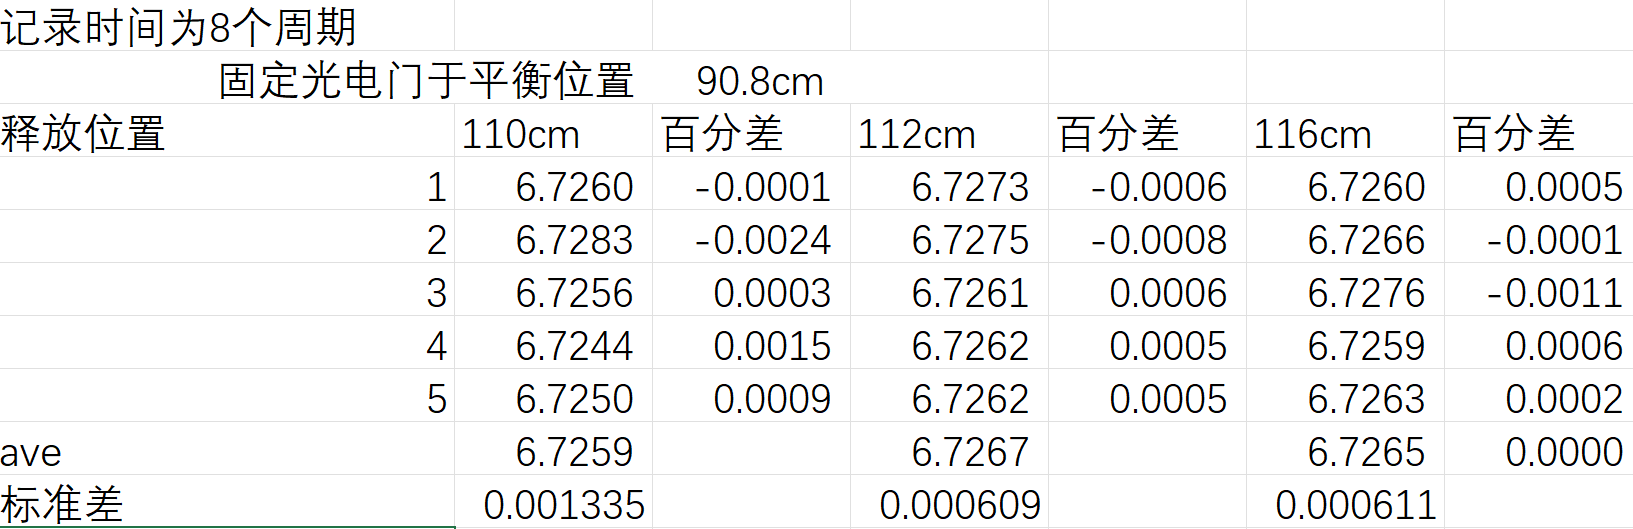
\includegraphics[height=0.3\textwidth,width=0.5\textwidth]{yanzhengwuguanshujv.png}
%     \caption{验证振动周期与初始状态无关数据处理}\label{yanzhengwuguanshujv}
%   \end{figure}
%   验证振动周期与初始状态无关实验的数据及数据处理如图\ref{yanzhengwuguanshujv}所展示的那样。每个数据和该
%   数据所在组平均值之间的相差不超过0.01s,除以八个周期后近似可以为相等,标准差也小于0.01。能验证振动周期与
%   初始状态无关。

%   实验中的误差可能来源于
  
%   1、每次释放位置不能保证完全相同

%   2、光电门传感器精度限制,以及挡光板的宽度

%   3、实验中气垫滑轨不能保证完全水平,出现倾斜

%   \subsection{验证周期公式$T=2\pi \sqrt{\frac{m}{k}}$}
%   \begin{figure}[b]
%     \centering
%     \begin{minipage}[b]{0.48\textwidth}
%       \centering
%       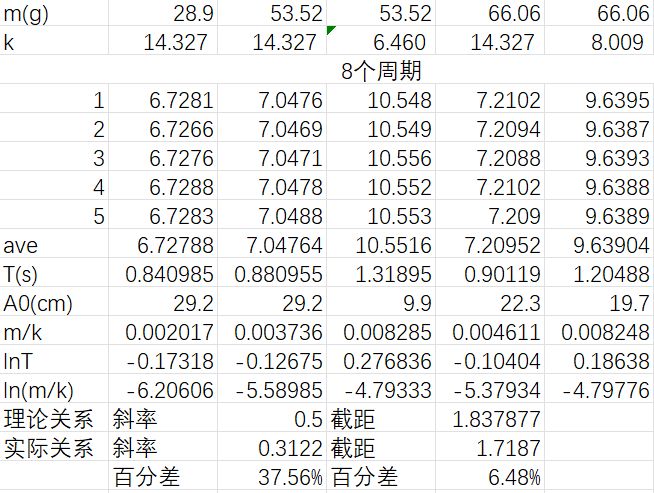
\includegraphics[width=0.46\textwidth]{yanzhengzhouqihanshu.png}
%       \caption{验证周期公式$T=2\pi \sqrt{\frac{m}{k}}$实验数据}\label{yanzhengzhouqihanshu}
%     \end{minipage}
%     \begin{minipage}[b]{0.48\textwidth}
%       \centering
%       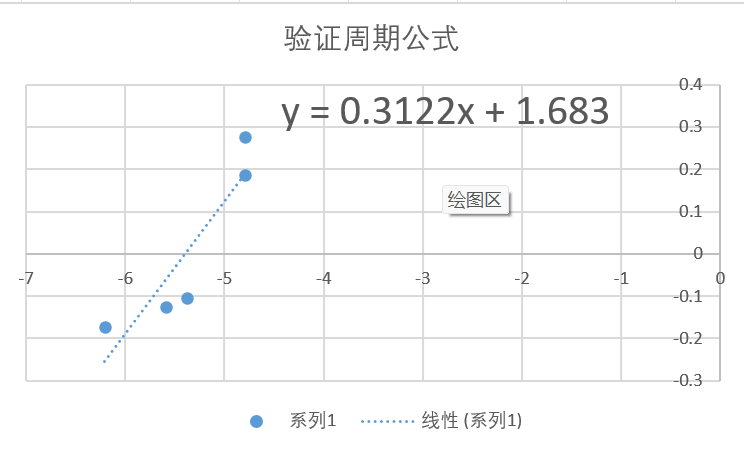
\includegraphics[width=0.46\textwidth]{yanzhengzhouqihanshuzuotu.png}
%       \caption{验证周期公式$T=2\pi \sqrt{\frac{m}{k}}$数据处理}\label{yanzhengzhouqigongshizuotu}
%     \end{minipage}
%   \end{figure}
%   验证周期公式的实验数据如图\ref{yanzhengzhouqihanshu}所示,实验数据处理如图\ref{yanzhengzhouqigongshizuotu}
%   所示那样。本实验误差较大,涉及不确定度较多。
%   实验中理论图像的斜率等于$\frac{1}{2}$,实验中理论截距为$\ln{2\pi}$。实际实验中图像的
%   斜率等于$0.3122$,实际截距为$1.7187$。
%   实验中理论和实际数据的百分差,斜率为$37.56\%$,截距为$6.48\%$

%   实验中的误差可能来源于 
  
%   1、每次释放位置不能保证完全相同

%   2、光电门传感器精度限制,以及挡光板的宽度引入的误差。同时涉及质量称量,引入新的误差

%   3、实验中气垫滑轨不能保证完全水平,出现倾斜

%   实验中理论和实际的误差比较大,需要更多数据及更进一步的实验。其中斜率的误差较截距较大。
% \newpage

% \section{思考题}
%   \subsection{小灯泡不发光的时候电阻为“冷态电阻”。设计实验测得冷态电阻}

%   \subsection{如何根据实验数据获得pn结$I-U$关系经验公式}

%   \subsection{如何采用光学方法测量并获得发光二极管的峰值波长}

%   \subsection{如果使用示波器直接观察稳压二极管的伏安特性曲线,在本实验基础上需要增加什么装置。对比试验并列出说明关键操作步骤}
% \newpage

\section{实验中个人的思考与感想}
  \subsection{对于实验个人观点}

  \subsection{实验中的总结}



\end{document}